% \iffalse meta-comment
%
% Copyright (C) 2017 by Scott Pakin <scott+hyxmp@pakin.org>
% -------------------------------------------------------
%
% This file may be distributed and/or modified under the
% conditions of the LaTeX Project Public License, either version 1.3c
% of this license or (at your option) any later version.
% The latest version of this license is in:
%
%    http://www.latex-project.org/lppl.txt
%
% and version 1.3c or later is part of all distributions of LaTeX
% version 2008/05/04 or later.
%
% \fi
%
% \iffalse
%<*driver>
\ProvidesFile{hyperxmp.dtx}
%</driver>
%<package>\NeedsTeXFormat{LaTeX2e}[1999/12/01]
%<package>\ProvidesPackage{hyperxmp}
%<*package>
    [2017/02/23 v3.2 Store hyperref metadata in XMP format]
%</package>
%
%<*driver>
\bgroup
  \catcode`\&=11
  \gdef\levelchar{&}
\egroup
\documentclass{ltxdoc}
\usepackage{graphicx}
\usepackage{color}
\usepackage{tocbibind}
\usepackage{microtype}
\usepackage{needspace}
\usepackage{varioref}
\usepackage{alltt}
\usepackage{needspace}
\usepackage{hyperxmp}
\usepackage[bookmarksopen,bookmarksopenlevel=2,bookmarksnumbered]{hyperref}
\EnableCrossrefs
\CodelineIndex
\RecordChanges

% Specify this document's metadata.
\title{The \pkgname{hyperxmp} package\thanks{This document
  corresponds to \pkgname{hyperxmp}~\fileversion, dated \filedate.}}
\author{Scott Pakin \\ \texttt{scott+hyxmp@pakin.org}}
\hypersetup{%
  pdfauthor={Scott Pakin},
  pdftitle={The hyperxmp package},
  pdfsubject={LaTeX2e support for XMP metadata},
  pdfkeywords={LaTeX, embedded metadata, XMP, PDF, copyright, license, comments},
  pdfcopyright={Copyright (C) 2017, Scott Pakin},
  pdflicenseurl={http://www.latex-project.org/lppl/},
  pdfcaptionwriter={Scott Pakin},
  pdfcontactemail={scott+hyxmp@pakin.org},
  pdfcontacturl={http://www.pakin.org/\xmptilde scott/},
  pdflang={en-US},
  baseurl={http://mirror.ctan.org/macros/latex/contrib/hyperxmp/hyperxmp.pdf}
}

\begin{document}
  \DocInput{hyperxmp.dtx}
  \Needspace{10\baselineskip}
  \phantomsection\addcontentsline{toc}{section}{Change History}
  \PrintChanges
  \makeatletter
  \let\orig@index@prologue=\index@prologue
  \def\index@prologue{%
    \phantomsection\addcontentsline{toc}{section}{Index}
    \orig@index@prologue
  }%
  \makeatother
  \Needspace{12\baselineskip}
  \PrintIndex
\end{document}
%</driver>
% \fi
%
% \CheckSum{1775}
%
% \CharacterTable
%  {Upper-case    \A\B\C\D\E\F\G\H\I\J\K\L\M\N\O\P\Q\R\S\T\U\V\W\X\Y\Z
%   Lower-case    \a\b\c\d\e\f\g\h\i\j\k\l\m\n\o\p\q\r\s\t\u\v\w\x\y\z
%   Digits        \0\1\2\3\4\5\6\7\8\9
%   Exclamation   \!     Double quote  \"     Hash (number) \#
%   Dollar        \$     Percent       \%     Ampersand     \&
%   Acute accent  \'     Left paren    \(     Right paren   \)
%   Asterisk      \*     Plus          \+     Comma         \,
%   Minus         \-     Point         \.     Solidus       \/
%   Colon         \:     Semicolon     \;     Less than     \<
%   Equals        \=     Greater than  \>     Question mark \?
%   Commercial at \@     Left bracket  \[     Backslash     \\
%   Right bracket \]     Circumflex    \^     Underscore    \_
%   Grave accent  \`     Left brace    \{     Vertical bar  \|
%   Right brace   \}     Tilde         \~}
%
%
% \changes{v1.0}{2006/05/14}{Initial version}
% \changes{v2.0}{2012/08/02}{Heiko Oberdiek's major rewrite of the code
%   to better support native-Unicode \string\TeX\ implementations
%   (\string\XeTeX\ and \string\LuaTeX)}
% \changes{v2.0}{2012/08/26}{Added support for the \protect\acro{XMP} Basic
%   schema and miscellaneous other bits of metadata}
% \changes{v1.2}{2010/06/04}{Added support for the \protect\XeTeX\ backend
%   (\texttt{xdvipdfmx})}
% \changes{v1.2}{2010/06/07}{Added support for the Photoshop schema}
% \changes{v2.2}{2010/12/06}{Added support for the \protect\acro{IPTC} Photo Metadata schema}
% \changes{v2.4}{2013/12/21}{Added support for the \protect\acro{PDF/A}
%   Identification schema, as requested by Florian Breitwieser}
% \changes{v2.5}{2014/06/19}{Enabled ``\texttt{\string\string\string\_}''
%   to work within email addresses, as requested by Leonid Sinev}
% \changes{v2.6}{2014/09/24}{Added support for a new \protect\optname{pdfdate}
%   key to explicitly specify the document date (and optionally time)}
% \changes{v2.9}{2016/04/25}{Force inclusion of \protect\xmpterm{dc:creator},
%   \protect\xmpterm{dc:title}, and \protect\xmpterm{dc:description}---even if
%   empty---when \protect\pkgname{hyperref} is loaded with the
%   \protect\optname{pdfa} option (suggested by Leonid Sinev)}
% \changes{v2.9}{2016/04/26}{Introduced the \protect\optname{pdftype}
%   package option, which enables an author to specify the type of
%   document being produced}
% \changes{v3.0}{2016/07/02}{Made the code compatible with \string\LuaTeX~0.85.
%   Thanks to Robert Schlicht, Leonid Sinev, and David Carlisle for bug
%   reports and to Leonid Sinev for helping test the new
%   \protect\pkgname{hyperxmp} code}
%
% \GetFileInfo{hyperxmp.dtx}
%
% \DoNotIndex{,\,\ ,\!,\",\#,\(,\),\*,\<,\>,\@cons,\@empty}
% \DoNotIndex{\@ifpackageloaded,\@ifundefined,\@nil,\@tempcnta,\@tempcntb}
% \DoNotIndex{\MessageBreak,\\,\^,\^,\_,\advance,\afterassignment}
% \DoNotIndex{\aftergroup,\begin,\begingroup,\bgroup,\catcode,\csname,\def}
% \DoNotIndex{\divide,\edef,\egroup,\else,\end,\endcsname,\endgroup}
% \DoNotIndex{\expandafter,\fi,\futurelet,\g@addto@macro,\gdef,\global,\if}
% \DoNotIndex{\ifcase,\ifnum,\ifx,\immediate,\lccode,\let,\loop,\lowercase}
% \DoNotIndex{\multiply,\newcommand,\noexpand,\or,\relax,\repeat,\space}
% \DoNotIndex{\string,\the,\toks,\uccode,\uppercase,\usepackage,\xdef,\~}
%
% ^^A  Define a few logical styles.
% \DeclareRobustCommand{\term}[1]{#1\SortIndex{#1}{#1}}
% \DeclareRobustCommand{\pkgname}[1]{\mbox{\textsf{#1}}\SortIndex{#1}{\textsf{#1}}}
% \makeatletter
% \DeclareRobustCommand{\xmpterm}[2][]{^^A
%   \def\xmptermopt{#1}^^A
%   \ifx\xmptermopt\@empty
%     \mbox{\textsf{#2}}^^A
%   \else
%     \mbox{\textsf{#2}}\slash\mbox{\textsf{#1}}^^A
%     \SortIndex{#1}{\textsf{#1}}^^A
%   \fi
%   \SortIndex{#2}{\textsf{#2}}^^A
% }
% \makeatother
% \DeclareRobustCommand{\pdfterm}[1]{\mbox{\textsf{#1}}\SortIndex{#1}{\textsf{#1}}}
% \DeclareRobustCommand{\cmdname}[1]{\mbox{\texttt{#1}}\SortIndex{#1}{\texttt{#1}}}
% \DeclareRobustCommand{\optname}[1]{^^A
%   \mbox{\textsf{#1}}^^A
%   \SortIndex{#1}{\textsf{#1} (option)}^^A
%   \index{options&#1=\textsf{#1}}^^A
% }
% \DeclareRobustCommand{\acrostyle}[1]{\textsc{\MakeLowercase{#1}}}
% \DeclareRobustCommand{\acro}[1]{^^A
%   \mbox{\acrostyle{#1}}^^A
%   \SortIndex{#1}{\acrostyle{#1}}^^A
% }
%
% ^^A  Define some other shortcut macros.
% \DeclareRobustCommand{\tex}{^^A
%   \texorpdfstring{\TeX\SortIndex{TeX}{\TeX}}{TeX}^^A
% }
% \DeclareRobustCommand{\XeTeXlogo}{^^A
%   X\lower0.5ex\hbox{\kern-.15em\reflectbox{E}}\kern-0.1667em\TeX
% }
% \DeclareRobustCommand{\XeTeX}{^^A
%   \texorpdfstring{\XeTeXlogo\SortIndex{XeTeX}{\XeTeXlogo}}{XeTeX}^^A
% }
% \DeclareRobustCommand{\XeLaTeXlogo}{^^A
%   X\lower0.5ex\hbox{\kern-.15em\reflectbox{E}}\kern-0.1667em\LaTeX
% }
% \DeclareRobustCommand{\XeLaTeX}{^^A
%   \texorpdfstring{\XeLaTeXlogo\SortIndex{XeLaTeX}{\XeLaTeXlogo}}{XeLaTeX}^^A
% }
% \DeclareRobustCommand{\LuaTeXlogo}{Lua\TeX}
% \DeclareRobustCommand{\LuaTeX}{^^A
%   \texorpdfstring{\LuaTeXlogo\SortIndex{LuaTeX}{\LuaTeXlogo}}{LuaTeX}^^A
% }
% \DeclareRobustCommand{\LuaLaTeXlogo}{Lua\LaTeX}
% \DeclareRobustCommand{\LuaLaTeX}{^^A
%   \texorpdfstring{\LuaLaTeXlogo\SortIndex{LuaLaTeX}{\LuaLaTeXlogo}}{LuaLaTeX}^^A
% }
% \DeclareRobustCommand{\pdfTeXlogo}{pdf\TeX}
% \DeclareRobustCommand{\pdfTeX}{^^A
%   \texorpdfstring{\pdfTeXlogo\SortIndex{pdfTeX}{\pdfTeXlogo}}{pdfTeX}^^A
% }
% \DeclareRobustCommand{\pdfLaTeXlogo}{pdf\LaTeX}
% \DeclareRobustCommand{\pdfLaTeX}{^^A
%   \texorpdfstring{\pdfLaTeXlogo\SortIndex{pdfLaTeX}{\pdfLaTeXlogo}}{pdfLaTeX}^^A
% }
% \DeclareRobustCommand{\Dvips}{^^A
%   \texorpdfstring{Dvips\SortIndex{dvips}{\texttt{dvips}}}{Dvips}^^A
% }
% \DeclareRobustCommand{\Lua}{^^A
%   Lua\index{Lua}^^A
% }
%
% ^^A  Define an environment just like macro but for Lua functions.
% \makeatletter
% \newenvironment{luafunc}{^^A
%   \begingroup
%     \catcode`\_=11
%     \def\PrintMacroName##1{\strut\MacroFont\string##1\ }^^A
%     \def\SpecialIndex@##1##2{^^A
%       \@bsphack
%       \special@index{\string##1\actualchar
%         \string\verb\quotechar*\verbatimchar##1\verbatimchar##2}^^A
%       \@esphack
%     }^^A
%     \begin{macro}^^A
% }{^^A
%     \end{macro}^^A
%   \endgroup
% }
% \makeatother
%
% ^^A  Pack figures a bit tighter onto the page.
% \renewcommand{\floatpagefraction}{0.8}
%
% ^^A  Help \pageref refer to arbitrary content.
% \newcounter{pagelabel}
%
% \maketitle
% \sloppy
%
% \begin{abstract}
%   \pkgname{hyperxmp} makes it easy for an author to include \acro{XMP}
%   metadata in a \acro{PDF} document produced by \LaTeX\@.  \pkgname{hyperxmp}
%   integrates seamlessly with \pkgname{hyperref} and requires virtually
%   no modifications to a document that already specifies document
%   metadata through \pkgname{hyperref}'s mechanisms.
% \end{abstract}
%
%
% \section{Introduction}
%
% Adobe Systems, Inc.\ has been promoting
% \acro{XMP}~\cite{Adobe2012:XMP}---eXtensible Metadata Platform---as a
% standard way to include metadata within a document.  The idea behind
% \acro{XMP} is that it is an \acro{XML}-based description of various
% document attributes and is embedded as uncompressed, unencoded text
% within the document it describes.  By storing the metadata this way it
% is independent of the document's file format.  That is, regardless of
% whether a document is in \acro{PDF}, \acrostyle{JPEG},
% \acrostyle{HTML}, or any other format, it is trivial for a program (or
% human) to locate, extract, and---using any standard \acro{XML}
% parser---process the embedded \acro{XMP} metadata.
%
% As of this writing there are few tools that actually do process
% \acro{XMP}\@.  However, it is easy to imagine future support existing
% in file browsers for displaying not only a document's filename but
% also its title, list of authors, description, and other metadata.
%
% \paragraph{This is too abstract!  Give me an example.}
% Consider a \LaTeX\ document with three authors: Jack Napier, Edward
% Nigma, and Harvey Dent.  The generated \acro{PDF} file will contain,
% among other information, the following stanza of \acro{XMP} code
% embedded within it:
%
% \begin{verbatim}
%    <dc:creator>
%      <rdf:Seq>
%        <rdf:li>Jack Napier</rdf:li>
%        <rdf:li>Edward Nigma</rdf:li>
%        <rdf:li>Harvey Dent</rdf:li>
%      </rdf:Seq>
%    </dc:creator>
% \end{verbatim}
%
% In the preceding code, the |dc| namespace refers to the
% \href{http://purl.org/DC/}{Dublin Core schema}, a collection of
% metadata properties.  The \xmpterm{dc:creator} property surrounds the
% list of authors.  The \textsf{rdf} namespace is the
% \href{http://www.w3.org/RDF/}{Resource Description Framework}, which
% defines \xmpterm{rdf:Seq} as an ordered list of values.  Each author
% is represented by an individual list item (\xmpterm{rdf:li}), making
% it easy for an \acro{XML} parser to separate the authors' names.
%
% Remember that \acro{XMP} code is stored as \emph{metadata}.  It does
% not appear when viewing or printing the \acro{PDF} file.  Rather, it
% is intended to make it easy for applications to identify and
% categorize the document.
%
% \paragraph{What metadata does \textsf{hyperxmp} process?}
% \pkgname{hyperxmp} knows how to embed all of the following types of
% metadata within a document:
%
% \begin{itemize} \raggedright
%   \item authors (\xmpterm{dc:creator})
%   \item base \acro{URL} (\xmpterm{xmp:BaseURL})
%   \item contact address
%     (\xmpterm[CiAdrExtadr]{Iptc4xmpCore:CreatorContactInfo},
%     \xmpterm[CiAdrCity]{Iptc4xmpCore:CreatorContactInfo},
%     \xmpterm[CiAdrRegion]{Iptc4xmpCore:CreatorContactInfo},
%     \xmpterm[CiAdrPcode]{Iptc4xmpCore:CreatorContactInfo}, and
%     \xmpterm[CiAdrCtry]{Iptc4xmpCore:CreatorContactInfo})
%   \item contact email address(es) (\xmpterm[CiEmailWork]{Iptc4xmpCore:CreatorContactInfo})
%   \item contact telephone number(s) (\xmpterm[CiTelWork]{Iptc4xmpCore:CreatorContactInfo})
%   \item contact \acro{URL}(s) (\xmpterm[CiUrlWork]{Iptc4xmpCore:CreatorContactInfo})
%   \item copyright (\xmpterm{dc:rights} and \xmpterm{xmpRights:Marked})
%   \item date (\xmpterm{dc:date}, \xmpterm{xmp:CreateDate},
%     \xmpterm{xmp:ModifyDate}, and \xmpterm{xmp:MetadataDate})
%   \item document identifier (\xmpterm{xmpMM:DocumentID})
%   \item document instance identifier (\xmpterm{xmpMM:InstanceID})
%   \item document type (\xmpterm{dc:type})
%   \item file format (\xmpterm{dc:format})
%   \item keywords (\xmpterm{pdf:Keywords} and \xmpterm{dc:subject})
%   \item language (\xmpterm{dc:language})
%   \item \LaTeX\ file name (\xmpterm{dc:source})
%   \item license \acro{URL} (\xmpterm{xmpRights:WebStatement})
%   \item metadata writer (\xmpterm{photoshop:CaptionWriter})
%   \item \acro{PDF} version (\xmpterm{pdf:PDFVersion})
%   \item \acro{PDF}-generating tool (\xmpterm{pdf:Producer} and \xmpterm{xmp:CreatorTool})
%   \item \acro{PDF/A} compliance level and version (\xmpterm{pdfaid:part} and \xmpterm{pdfaid:conformance})
%   \item primary author's position/title (\xmpterm{photoshop:AuthorsPosition})
%   \item summary (\xmpterm{dc:description})
%   \item title (\xmpterm{dc:title})
% \end{itemize}
%
% \noindent
% More types of metadata may be added in a future release.
%
% \paragraph{How does \textsf{hyperxmp} compare to the \textsf{xmpincl}
% package?}
% The short answer is that \pkgname{xmpincl} is more flexible but
% \pkgname{hyperxmp} is easier to use.  With \pkgname{xmpincl}, the
% author manually constructs a file of arbitrary \acro{XMP} data and the
% package merely embeds it within the generated \acro{PDF} file.  With
% \pkgname{hyperxmp}, the author specifies values for various predefined
% metadata types and the package formats those values as \acro{XMP} and embeds
% the result within the generated \acro{PDF} file.
%
% \pkgname{xmpincl} can embed \acro{XMP} only when running under \pdfLaTeX\ and
% only when in \acro{PDF}-generating mode.  \pkgname{hyperxmp} additionally
% works with a few other \acro{PDF}-producing \LaTeX\ backends.
%
% \pkgname{hyperxmp} and \pkgname{xmpincl} can complement each other.
% An author may want to use \pkgname{hyperxmp} to produce a basic set of
% \acro{XMP} code, then extract the \acro{XMP} code from the \acro{PDF} file with a text
% editor, augment the \acro{XMP} code with any metadata not supported by
% \pkgname{hyperxmp}, and use \pkgname{xmpincl} to include the modified
% \acro{XMP} code in the \acro{PDF} file.
%
% \section{Usage}
%
% \pkgname{hyperxmp} works by postprocessing some of the package options
% honored by \pkgname{hyperref}.  To use \pkgname{hyperxmp}, merely put
% a |\usepackage{hyperxmp}| in your document's preamble.  That line can
% appear anywhere before the \pkgname{hyperref} \acro{PDF} options are
% specified (i.e.,~with either |\usepackage[|\dots|]{hyperref}| or
% |\hypersetup{|\dots|}|).  \pkgname{hyperxmp} will construct its
% \acro{XMP} data using the following \pkgname{hyperref} options:
%
% \begin{itemize}
%   \item \optname{baseurl}
%   \item \optname{pdfauthor}
%   \item \optname{pdfcreationdate}
%   \item \optname{pdfkeywords}
%   \item \optname{pdflang}
%   \item \optname{pdfmoddate}
%   \item \optname{pdfproducer}
%   \item \optname{pdfsubject}
%   \item \optname{pdftitle}
% \end{itemize}
%
% \noindent
% \mbox{}\label{page:begin-new-options}
% \pkgname{hyperxmp} instructs \pkgname{hyperref} also to accept the
% following options, which have meaning only to \pkgname{hyperxmp}:
%
% \begin{itemize}
%   \item \optname{pdfaconformance}
%   \item \optname{pdfapart}
%   \item \optname{pdfauthortitle}
%   \item \optname{pdfcaptionwriter}
%   \item \optname{pdfcontactaddress}
%   \item \optname{pdfcontactcity}
%   \item \optname{pdfcontactcountry}
%   \item \optname{pdfcontactemail}
%   \item \optname{pdfcontactphone}
%   \item \optname{pdfcontactpostcode}
%   \item \optname{pdfcontactregion}
%   \item \optname{pdfcontacturl}
%   \item \optname{pdfcopyright}
%   \item \optname{pdfdate}
%   \item \optname{pdflicenseurl}
%   \item \optname{pdfmetadate}
%   \item \optname{pdfmetalang}
%   \item \optname{pdftype}
% \end{itemize}
% \label{page:end-new-options}
%
% The two most obscure---but alphabetically first---of the above,
% \optname{pdfaconformance} and \optname{pdfapart}, are used in
% conjunction with \pkgname{hyperref}'s \optname{pdfa} option to claim a
% particular \acro{PDF/A} standard by which the document abides.  They
% default to \optname{pdfapart}=|1| and \optname{pdfaconformance}=|B|,
% indicating the \acro{PDF/A}-\textsc{1b} standard.  These can be
% changed (with caution) to assert that the document abides by a
% different standard (e.g.,~\acro{PDF/A}-\textsc{2u}).
%
% \optname{pdfauthortitle} indicates the primary author's position or
% title.  \optname{pdfcaptionwriter} specifies the name of the person
% who added the metadata to the document.  The next eight items describe
% how to contact the person or institution responsible for the document
% (the ``contact'').  \optname{pdfcontactaddress} is the contact's
% street address and can include the institution name if the contact is
% an institution; \optname{pdfcontactcity} is the contact's city.
% \optname{pdfcontactcountry} is the contact's country;
% \optname{pdfcontactemail} is the contact's email address (or multiple,
% comma-separated email addresses); \optname{pdfcontactphone} is the
% contact's telephone number (or multiple, comma-separated telephone
% numbers); \optname{pdfcontactpostcode} is the contact's postal code;
% \optname{pdfcontactregion} is the contact's state or province; and
% \optname{pdfcontacturl} is the contact's \acro{URL} (or multiple,
% comma-separated \acro{URL}s).
%
% \acro{XMP} metadata can include a number of dates (in fact,
% timestamps, as they include both date and time components).
% \optname{pdfdate} specifies the document date.  It is analogous to the
% \LaTeX\ |\date| command, and, like |\date|, defaults to the date the
% document was built.  It must be specified in either \acro{XMP}
% format~\cite{Adobe2012:XMP} or \acro{PDF} format~\cite{Adobe2008:PDF}.
% \acro{XMP} dates are written in the form
% \textsc{yyyy}|-|\textsc{mm}|-|\textsc{dd}|T|hh|:|mm|:|ss|+|\textsc{tt}|:|tt.\footnote{Although
%   allowed by \acro{XMP}, \pkgname{hyperxmp} does not currently accept
%   fractions of a second in timestamps.}  A W3C
% recommendation~\cite{Wolf1997:date-time} discusses this format in more
% detail, but as an example, 14~hours, 15~minutes, 9~seconds past
% midnight U.S. Mountain Daylight Time (UTC-6) on the 23rd day of
% September in the year~2014 should be written as
% \texttt{2014-09-23T14:15:09-06:00}.  This can be truncated (with loss
% of information) to \texttt{2014-09-23T14:15:09} or
% \texttt{2014-09-23T14:15} or \texttt{2014-09-23} or \texttt{2014-09}
% or \texttt{2014} but no other subsets.  \acro{PDF} dates are written
% in the form |D:|\textsc{yyyymmdd}hhmmss|+|\textsc{tt}|'|tt|'|.  The
% same date in the preceding example would be written as
% \texttt{D:20140923141509-06'00'} in \acro{PDF} format.
%
% The document's creation date, modification date, and metadata date are
% normally set automatically, but \optname{pdfcreationdate},
% \optname{pdfmoddate}, and \optname{pdfmetadate} can be used to
% override the defaults.  Like \optname{pdfdate}, \optname{pdfmetadate}
% can be specified in either \acro{XMP} or \acro{PDF} format.  However,
% because \pkgname{hyperref} defines \optname{pdfcreationdate} and
% \optname{pdfmoddate} and expects these to be written as \acro{PDF}
% dates, \pkgname{hyperxmp} concomitantly accepts these two dates only
% in \acro{PDF} format as well.  Note that it's rare that a document
% would need to specify any of \optname{pdfcreationdate},
% \optname{pdfmoddate}, or \optname{pdfmetadate}.
%
% \optname{pdfcopyright} defines the copyright text, and
% \optname{pdflicenseurl} identifies a \acro{URL} that points to the
% document's license agreement.
%
% \optname{pdfmetalang} indicates the natural language in which the
% metadata is written, typically as an \acro{IETF} language
% tag~\cite{IANA2011:lang-tags}, for example, ``|en|'' for English,
% ``|en-US|'' for specifically United States English, ``|de|'' for
% German, and so forth.  If \optname{pdfmetalang} is not specified,
% \pkgname{hyperxmp} assumes the metadata language is the same as the
% document language (\pkgname{hyperref}'s \optname{pdflang} option).  If
% neither \optname{pdfmetalang} nor \optname{pdflang} is specified,
% \pkgname{hyperxmp} uses only ``|x-default|'' as the metadata language.
% Note that ``|x-default|'' metadata is always included in addition to
% the specified metadata language, as the user reading the document may
% not have specified a language preference.
%
% \optname{pdftype} describes the type of document being produced.  This
% refers to ``the nature or genre of the resource''~\cite{Adobe2012:XMP}
% such as ``|poem|'', ``|novel|'' or ``|working paper|'', as opposed to
% the file format (always ``|application/pdf|'' when generated by
% \pkgname{hyperxmp}).  Although \optname{pdftype} can be assigned an
% arbitrary piece of text, the \acro{XMP} specification recommends
% selecting types from a ``controlled vocabulary'' such as the DCMI Type
% Vocabulary~\cite{DCMI2012:meta-terms}.  The DCMI Type Vocabulary
% currently consists of only ``|Collection|'', ``|Dataset|'',
% ``|Event|'', ``|Image|'', ``|InteractiveResource|'',
% ``|MovingImage|'', ``|PhysicalObject|'', ``|Service|'',
% ``|Software|'', ``|Sound|'', ``|StillImage|'', and ``|Text|''.
% \optname{pdftype} defaults to ``|Text|'', which refers to ``books,
% letters, dissertations, poems, newspapers, articles, archives of
% mailing lists,''~\cite{DCMI2012:meta-terms} and other forms of
% text---all things \LaTeX\ is commonly used to typeset.
%
% It is usually more convenient to provide values for those options using
% \pkgname{hyperref}'s |\hypersetup| command than on the |\usepackage|
% command line.  See
% \href{http://mirrors.ctan.org/macros/latex/contrib/hyperref/hyperref.pdf}{the
% \pkgname{hyperref} manual} for more information.  The following is a
% sample \LaTeX\ document that provides values for most of the metadata
% options that \pkgname{hyperxmp} recognizes:
%
% \Needspace{4\baselineskip}
% \refstepcounter{pagelabel}
% \label{page:begin-sample-doc}
% \begin{verbatim}
%     \documentclass{article}
%     \usepackage{hyperxmp}
%     \usepackage{hyperref}
%     \title{%
%       On a heuristic viewpoint concerning the production and
%       transformation of light}
%     \author{Albert Einstein}
%     \date{March 17, 1905}
%     \hypersetup{%
%       pdftitle={%
%         On a heuristic viewpoint concerning the production and
%         transformation of light},
%       pdfauthor={Albert Einstein},
%       pdfauthortitle={Technical Assistant, Level III},
%       pdfdate={1905-03-17},
%       pdfcopyright={Copyright (C) 1905, Albert Einstein},
%       pdfsubject={photoelectric effect},
%       pdfkeywords={energy quanta, Hertz effect, quantum physics},
%       pdflicenseurl={http://creativecommons.org/licenses/by-nc-nd/3.0/},
%       pdfcaptionwriter={Scott Pakin},
%       pdfcontactaddress={Kramgasse 49},
%       pdfcontactcity={Bern},
%       pdfcontactpostcode={3011},
%       pdfcontactcountry={Switzerland},
%       pdfcontactphone={031 312 00 91},
%       pdfcontactemail={aeinstein@ipi.ch},
%       pdfcontacturl={%
%         http://einstein.biz/,
%         https://www.facebook.com/AlbertEinstein
%       },
%       pdflang={en},
%       baseurl={http://mirror.ctan.org/macros/latex/contrib/hyperxmp/}
%     }
%     \begin{document}
%     \maketitle
%     A profound formal difference exists between the theoretical
%     concepts that physicists have formed about gases and other
%     ponderable bodies, and Maxwell's theory of electromagnetic
%     processes in so-called empty space\dots
%     \end{document}
% \end{verbatim}
% \refstepcounter{pagelabel}
% \label{page:end-sample-doc}
%
% Compile the document to \acro{PDF} using any of the following
% approaches:
%
% \begin{itemize}
%   \item \pdfLaTeX
%   \item \LuaLaTeX
%   \item \LaTeX~$+$ Dvipdfm
%   \item \LaTeX~$+$ \Dvips~$+$ Adobe Acrobat Distiller
%   \item \XeLaTeX
% \end{itemize}
%
% \noindent
% Unfortunately, the \LaTeX~$+$ \Dvips~$+$ \term{Ghostscript} path
% doesn't work.
% \href{http://bugs.ghostscript.com/show_bug.cgi?id=690066}{Ghostscript
%   bug report~\#690066}, closed with ``\textsc{wontfix}'' status on
% 2012-05-28, explains that \term{Ghostscript} doesn't honor the
% \pdfterm{Metadata} tag needed to inject a custom \acro{XMP} packet.
% Instead, \term{Ghostscript} fabricates an \acro{XMP} packet of its own
% based on the metadata it finds in the \acro{PDF} file's \pdfterm{Info}
% dictionary (\pdfterm{Author}, \pdfterm{Title}, \pdfterm{Subject}, and
% \pdfterm{Keywords}).
%
% \bigskip
%
% Once the document is compiled, the resulting \acro{PDF} file will
% contain an \acro{XMP} packet that looks something like that shown in
% Appendix~\ref{sec:sample-packet}.  Figure~\ref{fig:xmp-metadata-1} is
% a screenshot of the \acro{XMP} metadata as it appears in Adobe
% Acrobat's ``Advanced'' metadata dialog box.  Further clicking on the
% ``Advanced'' item within that dialog box displays all of the
% document's metadata sorted by schema as shown in
% Figure~\ref{fig:xmp-metadata-2}.
%
% \begin{figure}[htbp]
%   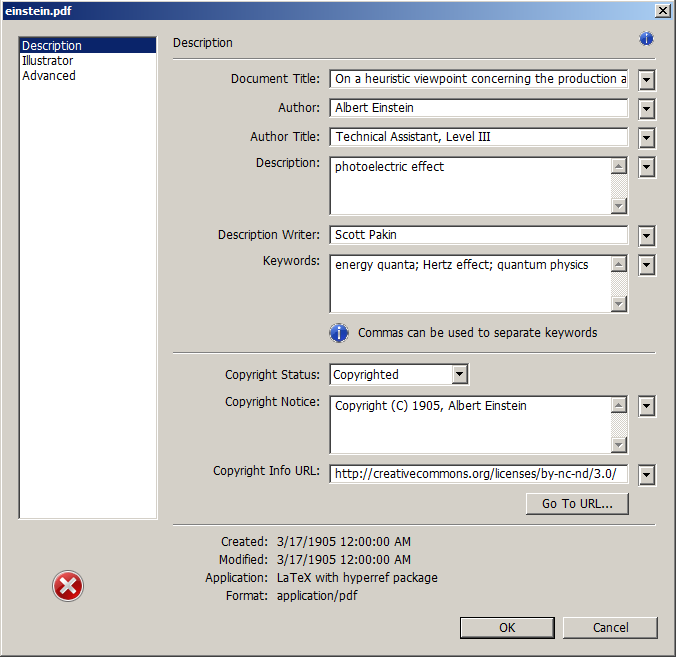
\includegraphics[width=\linewidth]{einstein1}
%   \caption{\acro{XMP} metadata as it appears in Adobe Acrobat}
%   \label{fig:xmp-metadata-1}
% \end{figure}
%
% \begin{figure}[htbp]
%   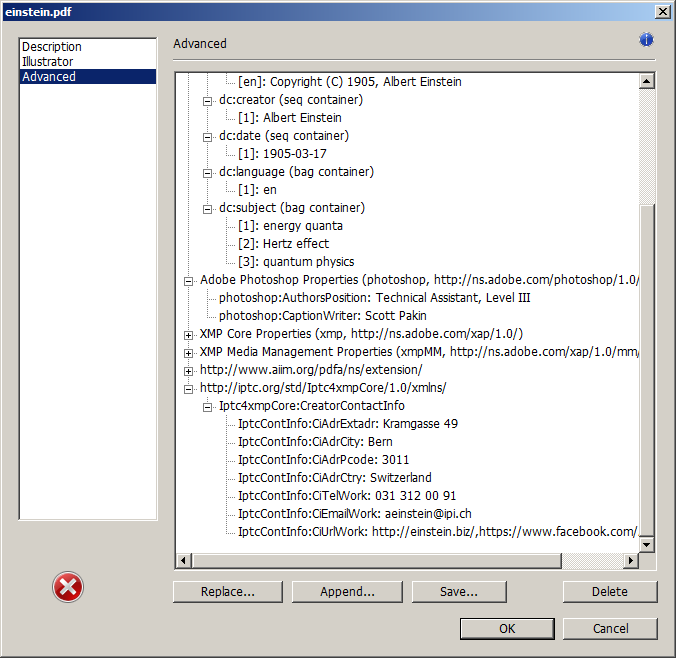
\includegraphics[width=\linewidth]{einstein2}
%   \caption{Additional \acro{XMP} metadata as it appears in Adobe Acrobat}
%   \label{fig:xmp-metadata-2}
% \end{figure}
%
% \paragraph{Note~1: Acrobat \pdfterm{Author} bug}
% \label{page:author-bug}
% A bug in Adobe Acrobat---at least in versions~10.0.1 and
% earlier---causes that \acro{PDF} reader to confuse the \acro{XMP} and
% non-\acro{XMP} author lists when displaying the document's metadata.
% Specifically, the first author is displayed as the concatenated list
% of authors from the non-\acro{XMP} data (\pdfterm{Author}) while the
% remaining authors are displayed from the \acro{XMP} data
% (\xmpterm{dc:creator}).  For example, suppose that a document's authors
% are Jack Napier, Edward Nigma, and Harvey Dent.  When displaying the
% document properties, Adobe Acrobat replaces ``Jack Napier'' with a
% single author named ``Jack Napier, Edward Nigma, Harvey Dent'' and
% leaves ``Edward Nigma'' and ``Harvey Dent'' as the second and third
% authors, respectively.
%
% \DescribeMacro{\XMPTruncateList}
% The \pkgname{hyperxmp} package provides a workaround for this bug in
% the form of the |\XMPTruncateList| macro.  |\XMPTruncateList| takes
% the name of a list (a \pkgname{hyperref} option name) and replaces the
% list with the value of its first element.  Currently, the only
% meaningful usage is to put
%
% \begin{verbatim}
%     \XMPTruncateList{pdfauthor}
% \end{verbatim}
%
% \noindent
% in your document's preamble.  This will cause Adobe Acrobat to
% properly display all of the authors but at the cost of other
% \acro{PDF} readers likely displaying only the first author.
%
%
% \paragraph{Note~2: Acrobat multiline-field bug}
% The \acro{IPTC} Photo Metadata schema states that ``the [contact]
% address is a multiline field''~\cite{IPTC2010:photo-meta}.
% \pkgname{hyperxmp} converts commas in \optname{pdfcontactaddress}'s
% argument to line breaks in the generated \acro{XML}\@.  Unfortunately,
% A bug in Adobe Acrobat---at least in versions~10.0.1 and
% earlier---causes that \acro{PDF} reader to discard line breaks in the
% contact address.  Interestingly, Adobe Illustrator CS5 correctly
% displays the contact address.
% \DescribeMacro{\xmplinesep}
% If you find Adobe Acrobat's behavior bothersome, you can redefine the
% |\xmplinesep| macro as a string to use as an address-line separator.
% For example, the following replaces all commas appearing in
% \optname{pdfcontactaddress}'s argument with semicolons:
%
% \begin{verbatim}
%     \renewcommand*{\xmlinesep}{;}
% \end{verbatim}
%
%
% \paragraph{Note~3: Object compression}
% One intention of \acro{XMP} is that metadata embedded in a file be
% readable even without knowledge of the file's format.  That is, the
% metadata are expected to appear as plain text.  Although
% \pkgname{hyperxmp} does its best to honor that intention, it faces
% a few challenges:
%
% \begin{enumerate}
% \item When run with versions of \LuaLaTeX\ earlier than 0.85,
%   \pkgname{hyperxmp} leaves all \acro{PDF} objects uncompressed.  This
%   is due to \LuaLaTeX\ treating object compression as a global
%   parameter, unlike \pdfLaTeX, which treats it as a local parameter.
%   Hence, when \pkgname{hyperxmp} requests that the \acro{XMP} packet
%   be left uncompressed, \LuaLaTeX\ in fact leaves \emph{all}
%   \acro{PDF} streams uncompressed.  Beginning with version~3.0,
%   \pkgname{hyperxmp} includes a workaround that correctly leaves only
%   the \acro{XMP} metadata uncompressed, but this workaround is
%   implemented only for \LuaLaTeX\ v0.85 onwards.
%
% \item \XeLaTeX\ (or, more precisely, the \cmdname{xdvipdfmx} back end)
%   exhibits the opposite problem.  It compresses \emph{all} \acro{PDF}
%   objects, including the ones containing \acro{XMP} metadata.  While
%   Adobe Acrobat can still detect and utilize the \acro{XMP} metadata,
%   non-\acro{PDF}-aware applications are unlikely to see the metadata.
%   Three options to consider are to (1)~use a different program
%   (e.g.,~\LuaLaTeX), (2)~pass the |--output-driver="xdvipdfmx -z0"|
%   option to \XeLaTeX\ to instruct \cmdname{xdvipdfmx} to turn off all
%   compression (which will of course make the \acro{PDF} file
%   substantially larger), or (3)~postprocess the generated \acro{PDF}
%   file by loading it into the commercial version of Adobe Acrobat and
%   re-saving it with the Save As\dots\ menu option.
% \end{enumerate}
%
%
% \paragraph{Note~4: Literal commas}
% \pkgname{hyperxmp} splits the \optname{pdfauthor} and
% \optname{pdfkeywords} lists at commas.  Therefore, when specifying
% \optname{pdfauthor} and \optname{pdfkeywords}, you should separate
% items with commas.  Also, omit ``|and|'' and other text that does not
% belong to any list item.  The following examples should serve as
% clarification:
%
% \begin{description}
%   \item[Wrong:] |pdfauthor={Jack Napier, Edward Nigma,|
%     \textcolor{red}{\texttt{and}} |Harvey Dent}|
%   \item[Wrong:] |pdfauthor={Jack Napier|\textcolor{red}{\texttt{;}}
%     |Edward Nigma|\textcolor{red}{\texttt{;}}
%     |Harvey Dent}|
%   \item[Right:] |pdfauthor={Jack Napier, Edward Nigma, Harvey Dent}|
% \end{description}
%
% \noindent
% \DescribeMacro{\xmpcomma}
% \DescribeMacro{\xmpquote}
% If you need to include a literal comma within an author or keyword
% list (where commas normally separate list items) or a street address
% (where commas normally separate lines), use the |\xmpcomma| macro to
% represent it, and wrap the entire entry containing the comma within
% |\xmpquote{|\dots|}| as shown below:
%
% \begin{verbatim}
%     pdfauthor={\xmpquote{Jack Napier\xmpcomma\ Jr.},
%                \xmpquote{Edward Nigma\xmpcomma\ PhD},
%                \xmpquote{Harvey Dent\xmpcomma\ Esq.}}
%
%     pdfcontactaddress={Office of the President,
%                        \xmpquote{Wayne Enterprises\xmpcomma\ Inc.},
%                        One Wayne Blvd}
% \end{verbatim}
%
% As of version~2.2 of \pkgname{hyperxmp}, it is acceptable to use
% |\xmpcomma| and |\xmpquote| within any \pkgname{hyperxmp} option, not
% just in those in which a comma normally serves as a separator
% (i.e.,~lists and multiline fields).  Outside of cases in which a comma
% serves as a separator, |\xmpcomma| is treated as an ordinary comma,
% and |\xmpquote| returns its argument unmodified.  Hence, it is
% legitimate to use |\xmpcomma| and |\xmpquote| in cases like the
% following
%
% \begin{verbatim}
%     pdfauthortitle={\xmpquote{Psychiatrist\xmpcomma\ Arkham Asylum}}
% \end{verbatim}
%
% \noindent
% (Like most \pkgname{hyperxmp} options, \optname{pdfauthortitle}
% inserts its argument unmodified in an \acro{XMP} tag.)  When in
% doubt, use |\xmpcomma| and |\xmpquote|; it should always be safe
% to do so.
%
% \DescribeMacro{\xmptilde}
% Version~2.4 of \pkgname{hyperxmp} introduces a convenience macro
% called |\xmptilde|.  |\xmptilde| expands to a literal tilde character
% instead of the nonbreaking space that ``|~|'' normally represents.
% Use it to represent \acro{URL}s such as
% \url{http://www.pakin.org/~scott/} (``|http://www.pakin.org/|\linebreak[0]|\xmptilde|
% |scott/|'') in options such as \optname{baseurl},
% \optname{pdfcontacturl} and \optname{pdflicenseurl}.
%
% \paragraph{Note~5: Unicode support}
% \term{Unicode} support is provided via the \pkgname{hyperref} package.
% If you specify \optname{unicode}|=true| either as a \pkgname{hyperref}
% option or as an argument to the |\hypersetup| command, the document
% can include \term{Unicode} characters in its \acro{XMP} fields.
%
% \paragraph{Note~6: Automatically specified metadata}
% \optname{pdftitle} defaults to the document's title as specified by
% |\title{|\dots|}|.  \optname{pdfauthor} defaults to the document's
% author(s) as specified by |\author{|\dots|}|.  \optname{pdfdate}
% defaults to the current date and time.  \optname{pdfmetalang}
% defaults to the same value as \optname{pdflang} if non-empty,
% ``|x-default|'' otherwise.  An implication of automatic
% metadata specification is that an author can simply include
% |\usepackage{hyperxmp}| in a document's preamble and benefit from
% a modicum of \acro{XMP} metadata with no additional effort.
%
%
% \StopEventually{^^A
% \section{Future Work}
% \label{sec:future-work}
%
% \paragraph{Help wanted}
% Ideally, \texttt{\string\xmpquote} should automatically replace all
% commas with \texttt{\string\xmpcomma}.  Unfortunately, my \tex\ skills
% are insufficient to pull that off.  If you know a way to make
% \texttt{\string\xmpquote\string{Hello, world\string}} work with both
% \term{Unicode} and non-\term{Unicode} encodings and with all
% \tex\ engines (\pdfTeX, \LuaTeX, \XeTeX, etc.), please send me a code
% patch.
%
% \appendix
%
% \section{Sample XMP packet}
% \label{sec:sample-packet}
%
% The following is an example of a complete \acro{XMP} packet as may be
% produced by \pkgname{hyperxmp}.  This packet corresponds to the
% metadata included in the sample \LaTeX\ document presented
% \vpagerefrange{page:begin-sample-doc}{page:end-sample-doc}.  For
% clarity, metadata values, either specified explicitly by the document
% or introduced automatically by \pkgname{hyperxmp}, are colored blue.
%
% ^^A  Color-code metadata values.
\newcommand{\metavalue}[1]{\textcolor{blue}{#1}}

^^A  Provide access to today's date, as formatted by hyperxmp.sty.
\makeatletter
\let\todayISO=\hyxmp@today
\makeatother

\begin{alltt}
    <?xpacket begin="\string\357\string\273\string\277" id="W5M0MpCehiHzreSzNTczkc9d"?>
    <x:xmpmeta xmlns:x="adobe:ns:meta/" x:xmptk="3.1-702">
       <rdf:RDF xmlns:rdf="http://www.w3.org/1999/02/22-rdf-syntax-ns#">
          <rdf:Description rdf:about=""
               xmlns:pdf="http://ns.adobe.com/pdf/1.3/">
               <pdf:Keywords>
                 \metavalue{energy quanta, Hertz effect, quantum physics}
               </pdf:Keywords>
               <pdf:Producer>\metavalue{pdfTeX-1.40.10}</pdf:Producer>
          </rdf:Description>
          <rdf:Description rdf:about=""
               xmlns:xmpRights="http://ns.adobe.com/xap/1.0/rights/">
             <xmpRights:Marked>\metavalue{True}</xmpRights:Marked>
             <xmpRights:WebStatement>
               \metavalue{http://creativecommons.org/licenses/by-nc-nd/3.0/}
             </xmpRights:WebStatement>
          </rdf:Description>
          <rdf:Description rdf:about=""
                xmlns:dc="http://purl.org/dc/elements/1.1/">
             <dc:format>\metavalue{application/pdf}</dc:format>
             <dc:title>
                <rdf:Alt>
                   <rdf:li xml:lang="en">
                     \metavalue{On a heuristic viewpoint concerning the production and
                     transformation of light}
                   </rdf:li>
                   <rdf:li xml:lang="x-default">
                     \metavalue{On a heuristic viewpoint concerning the production and
                     transformation of light}
                   </rdf:li>
                </rdf:Alt>
             </dc:title>
             <dc:description>
                <rdf:Alt>
                   <rdf:li xml:lang="en">\metavalue{photoelectric effect}</rdf:li>
                   <rdf:li xml:lang="x-default">\metavalue{photoelectric effect}</rdf:li>
                </rdf:Alt>
             </dc:description>
             <dc:rights>
                <rdf:Alt>
                   <rdf:li xml:lang="en">
                     \metavalue{Copyright (C) 1905, Albert Einstein}
                   </rdf:li>
                   <rdf:li xml:lang="x-default">
                     \metavalue{Copyright (C) 1905, Albert Einstein}
                   </rdf:li>
                </rdf:Alt>
             </dc:rights>
             <dc:creator>
                <rdf:Seq>
                   <rdf:li>\metavalue{Albert Einstein}</rdf:li>
                </rdf:Seq>
             </dc:creator>
             <dc:subject>
                <rdf:Bag>
                   <rdf:li>\metavalue{energy quanta}</rdf:li>
                   <rdf:li>\metavalue{Hertz effect}</rdf:li>
                   <rdf:li>\metavalue{quantum physics}</rdf:li>
                </rdf:Bag>
             </dc:subject>
             <dc:date>
                <rdf:Seq>
                   <rdf:li>\metavalue{1905-03-17}</rdf:li>
                </rdf:Seq>
             </dc:date>
             <dc:language>
                <rdf:Bag>
                   <rdf:li>\metavalue{en}</rdf:li>
                </rdf:Bag>
              </dc:language>
              <dc:type>
                 <rdf:Bag>
                    <rdf:li>\metavalue{Text}</rdf:li>
                 </rdf:Bag>
              </dc:type>
             <dc:source>\metavalue{einstein.tex}</dc:source>
          </rdf:Description>
          <rdf:Description rdf:about=""
                xmlns:photoshop="http://ns.adobe.com/photoshop/1.0/">
             <photoshop:AuthorsPosition>
               \metavalue{Technical Assistant, Level III}
             </photoshop:AuthorsPosition>
             <photoshop:CaptionWriter>\metavalue{Scott Pakin}</photoshop:CaptionWriter>
          </rdf:Description>
          <rdf:Description rdf:about=""
              xmlns:pdfaExtension="http://www.aiim.org/pdfa/ns/extension/"
              xmlns:pdfaSchema="http://www.aiim.org/pdfa/ns/schema#"
              xmlns:pdfaProperty="http://www.aiim.org/pdfa/ns/property#"
              xmlns:pdfaType="http://www.aiim.org/pdfa/ns/type#"
              xmlns:pdfaField="http://www.aiim.org/pdfa/ns/field#">
            <pdfaExtension:schemas>
              <rdf:Bag>
                <rdf:li rdf:parseType="Resource">
                  <pdfaSchema:schema>IPTC Core Schema</pdfaSchema:schema>
                  <pdfaSchema:namespaceURI>http://iptc.org/std/Iptc4xmpCore/1.0/xmlns/</pdfaSchema:namespaceURI>
                  <pdfaSchema:prefix>Iptc4xmpCore</pdfaSchema:prefix>
                  <pdfaSchema:property>
                    <rdf:Seq>
                      <rdf:li rdf:parseType="Resource">
                        <pdfaProperty:name>CreatorContactInfo</pdfaProperty:name>
                        <pdfaProperty:valueType>contactinfo</pdfaProperty:valueType>
                        <pdfaProperty:category>external</pdfaProperty:category>
                        <pdfaProperty:description>contact information for the document's creator</pdfaProperty:description>
                      </rdf:li>
                    </rdf:Seq>
                  </pdfaSchema:property>
                  <pdfaSchema:valueType>
                    <rdf:Seq>
                      <rdf:li rdf:parseType="Resource">
                        <pdfaType:type>contactinfo</pdfaType:type>
                        <pdfaType:namespaceURI>http://iptc.org/std/Iptc4xmpCore/1.0/xmlns/</pdfaType:namespaceURI>
                        <pdfaType:prefix>Iptc4xmpCore</pdfaType:prefix>
                        <pdfaType:description>contact information</pdfaType:description>
                        <pdfaType:field>
                          <rdf:Seq>
                            <rdf:li rdf:parseType="Resource">
                              <pdfaField:name>CiAdrExtadr</pdfaField:name>
                              <pdfaField:valueType>Text</pdfaField:valueType>
                              <pdfaField:description>contact address</pdfaField:description>
                            </rdf:li>
                            <rdf:li rdf:parseType="Resource">
                              <pdfaField:name>CiAdrCity</pdfaField:name>
                              <pdfaField:valueType>Text</pdfaField:valueType>
                              <pdfaField:description>contact city</pdfaField:description>
                            </rdf:li>
                            <rdf:li rdf:parseType="Resource">
                              <pdfaField:name>CiAdrRegion</pdfaField:name>
                              <pdfaField:valueType>Text</pdfaField:valueType>
                              <pdfaField:description>contact region</pdfaField:description>
                            </rdf:li>
                            <rdf:li rdf:parseType="Resource">
                              <pdfaField:name>CiAdrPcode</pdfaField:name>
                              <pdfaField:valueType>Text</pdfaField:valueType>
                              <pdfaField:description>contact postal code</pdfaField:description>
                            </rdf:li>
                            <rdf:li rdf:parseType="Resource">
                              <pdfaField:name>CiAdrCtry</pdfaField:name>
                              <pdfaField:valueType>Text</pdfaField:valueType>
                              <pdfaField:description>contact country</pdfaField:description>
                            </rdf:li>
                            <rdf:li rdf:parseType="Resource">
                              <pdfaField:name>CiTelWork</pdfaField:name>
                              <pdfaField:valueType>Text</pdfaField:valueType>
                              <pdfaField:description>contact telephone number</pdfaField:description>
                            </rdf:li>
                            <rdf:li rdf:parseType="Resource">
                              <pdfaField:name>CiEmailWork</pdfaField:name>
                              <pdfaField:valueType>Text</pdfaField:valueType>
                              <pdfaField:description>contact email address</pdfaField:description>
                            </rdf:li>
                            <rdf:li rdf:parseType="Resource">
                              <pdfaField:name>CiUrlWork</pdfaField:name>
                              <pdfaField:valueType>Text</pdfaField:valueType>
                              <pdfaField:description>contact url</pdfaField:description>
                            </rdf:li>
                          </rdf:Seq>
                        </pdfaType:field>
                      </rdf:li>
                    </rdf:Seq>
                  </pdfaSchema:valueType>
                </rdf:li>
              </rdf:Bag>
            </pdfaExtension:schemas>
          </rdf:Description>
          <rdf:Description rdf:about=""
               xmlns:Iptc4xmpCore="http://iptc.org/std/Iptc4xmpCore/1.0/xmlns/">
           <Iptc4xmpCore:CreatorContactInfo rdf:parseType="Resource">
             <Iptc4xmpCore:CiAdrExtadr>\metavalue{Kramgasse 49}</Iptc4xmpCore:CiAdrExtadr>
             <Iptc4xmpCore:CiAdrCity>\metavalue{Bern}</Iptc4xmpCore:CiAdrCity>
             <Iptc4xmpCore:CiAdrPcode>\metavalue{3011}</Iptc4xmpCore:CiAdrPcode>
             <Iptc4xmpCore:CiAdrCtry>\metavalue{Switzerland}</Iptc4xmpCore:CiAdrCtry>
             <Iptc4xmpCore:CiTelWork>\metavalue{031 312 00 91}</Iptc4xmpCore:CiTelWork>
             <Iptc4xmpCore:CiEmailWork>\metavalue{aeinstein@ipi.ch}</Iptc4xmpCore:CiEmailWork>
             <Iptc4xmpCore:CiUrlWork>
               \metavalue{http://einstein.biz/,
               https://www.facebook.com/AlbertEinstein}
             </Iptc4xmpCore:CiUrlWork>
           </Iptc4xmpCore:CreatorContactInfo>
          </rdf:Description>
          <rdf:Description rdf:about=""
                xmlns:xmp="http://ns.adobe.com/xap/1.0/">
             <xmp:CreateDate>\metavalue{\todayISO}</xmp:CreateDate>
             <xmp:ModifyDate>\metavalue{\todayISO}</xmp:ModifyDate>
             <xmp:MetadataDate>\metavalue{\todayISO}</xmp:MetadataDate>
             <xmp:CreatorTool>\metavalue{LaTeX with hyperref package}</xmp:CreatorTool>
             <xmp:BaseURL>
               \metavalue{http://mirror.ctan.org/macros/latex/contrib/hyperxmp/}
             </xmp:BaseURL>
          </rdf:Description>
          <rdf:Description rdf:about=""
                xmlns:xmpMM="http://ns.adobe.com/xap/1.0/mm/">
             <xmpMM:DocumentID>
               \metavalue{uuid:0595fdce-41dc-e4c4-6c418dc4ce46}
             </xmpMM:DocumentID>
             <xmpMM:InstanceID>
               \metavalue{uuid:efd754c4-1d7f-200a-ef754ce413ea}
             </xmpMM:InstanceID>
          </rdf:Description>
       </rdf:RDF>
    </x:xmpmeta>
    <?xpacket end="w"?>
\end{alltt}

%
% \begin{thebibliography}{1}
% \bibitem{Adobe2010:pdfmark}
% Adobe Systems, Inc., San Jose, California.
% \newblock {\em {A}dobe {A}crobat~{X} {SDK} Help, pdfmark Reference}.
% \newblock Available from
%   \url{http://www.adobe.com/devnet/acrobat/documentation.html}.
%
% \bibitem{Adobe1996:postscript}
% {Adobe Systems, Inc.}
% \newblock {\em {P}ost{S}cript Language Reference Manual}.
% \newblock Addison-Wesley, 2nd edition, January 1996, ISBN: \mbox{0-201-18127-4}.
%
% \bibitem{Adobe2008:PDF}
% Adobe Systems, Inc., San Jose, California.
% \newblock {\em Document Management---Portable Document Format---Part 1:
%   PDF~1.7}, July 2008.
% \newblock ISO \mbox{32000-1} standard document. Available from
%   \url{http://wwwimages.adobe.com/www.adobe.com/content/dam/Adobe/en/devnet/pdf/pdfs/PDF32000_2008.pdf}.
%
% \bibitem{Adobe2012:XMP}
% Adobe Systems, Inc., San Jose, California.
% \newblock {\em {XMP} Specification Part~1: Data model, Serialization, and Core
%   Properties}, April 2012.
% \newblock Available from
%   \url{http://wwwimages.adobe.com/www.adobe.com/content/dam/Adobe/en/devnet/xmp/pdfs/cc-201306/XMPSpecificationPart1.pdf}.
%
% \bibitem{DCMI2012:meta-terms}
% DCMI Usage Board
% \newblock {\em DCMI Metadata Terms}, June~14, 2012.
% \newblock Available from \url{http://dublincore.org/documents/dcmi-terms/}.
%
% \bibitem{Downes1994:ATB15}
% Michael Downes.
% \newblock Around the bend~\#15, answers, 4th (last) installment.
% \newblock \href{news:comp.text.tex}{\texttt{comp.text.tex}} newsgroup posting,
%   January~3, 1994.
% \newblock Archived by Google at
%   \url{http://groups.google.com/group/comp.text.tex/msg/7da7643b9e8f3b48}.
%
% \bibitem{IPTC2010:photo-meta}
% International Press Telecommunications Council.
% \newblock {\em {IPTC} Photo Metadata: Core 1.1/Extension 1.1}, July 2010.
% \newblock Revision~1. Available from
%   \url{http://www.iptc.org/std/photometadata/specification/IPTC-PhotoMetadata-201007_1.pdf}.
%
% \bibitem{IANA2011:lang-tags}
% {Internet Assigned Numbers Authority}.
% \newblock Language subtag registry, January~11, 2011.
% \newblock Available from
%   \url{http://www.iana.org/assignments/language-subtag-registry}.
%
% \bibitem{Leach2005:uuid}
% Paul~J. Leach, Michael Mealling, and Rich Salz.
% \newblock A {U}niversally {U}nique {ID}entifier ({UUID}) {URN} namespace.
% \newblock Request for Comments 4122, Internet Engineering Task Force, Network
%   Working Group, July 2005.
% \newblock Category: Standards Track. Available from
%   \url{http://www.ietf.org/rfc/rfc4122.txt}.
%
% \bibitem{PDFA2008:xmp-props}
% PDF/A Competence Center, Berlin, Germany.
% \newblock {\em {T}ech{N}ote~0008: Predefined {XMP} Properties in {PDF/A-1}},
%   March~20, 2008.
% \newblock Available from
%   \url{http://www.pdfa.org/wp-content/uploads/2011/08/tn0008_predefined_xmp_properties_in_pdfa-1_2008-03-20.pdf}.
%
% \bibitem{PDFA2008:ext-schemas}
% PDF/A Competence Center, Berlin, Germany.
% \newblock {\em {T}ech{N}ote~0009: {XMP} Extension Schemas in {PDF/A-1}},
%   March~20, 2008.
% \newblock Available from
%   \url{http://www.pdfa.org/wp-content/uploads/2011/08/tn0009_xmp_extension_schemas_in_pdfa-1_2008-03-20.pdf}.
%
% \bibitem{Wolf1997:date-time}
% Misha Wolf and Charles Wicksteed.
% \newblock Date and time formats.
% \newblock Note NOTE-datetime, World Wide Web Consortium (W3C), September~15,
%   1997.
% \newblock Available from \url{http://www.w3.org/TR/NOTE-datetime}.
% \end{thebibliography}
% }
%
%
% \section{Implementation}
%
% This section presents the commented \LaTeX\ source code for
% \pkgname{hyperxmp}.  Read this section only if you want to learn how
% \pkgname{hyperxmp} is implemented.
%
%
% \subsection{Initial preparation}
% \label{sec:initial-prep}
%
% \changes{v1.2}{2011/04/17}{Made the package compatible with \pkgname{ngerman}.
%   Thanks to Tobias Mueller for the bug report.}
%
% \begin{macro}{\hyxmp@dq@code}
% The \pkgname{ngerman} package redefines
% ``\,{\fontencoding{T1}\selectfont\textquotedbl}\,'' as an active
% character, which causes problems for \pkgname{hyperxmp} when it tries
% to use that character.  We therefore save the double-quote character's
% current category code in |\hyxmp@dq@code| and mark the character as
% category code~12 (``other'').  The original category code is restored
% at the end of the package code (Section~\ref{sec:clean-up}).
%    \begin{macrocode}
\edef\hyxmp@dq@code{\the\catcode`\"}
\catcode`\"=12
%    \end{macrocode}
% \end{macro}
%
% \changes{v1.5}{2012/03/10}{Made the \protect\acro{XMP} inclusion more robust.
%   Thanks to Heiko Oberdiek for the bug report and suggested modifications.}
%
% \begin{macro}{\hyxmp@at@end}
% \begin{macro}{\hyxmp@driver}
% The |\hyxmp@at@end| macro includes code at the end of the document.
% For \pdfTeX, the standard |\AtEndDocument| works well enough.  For all
% the other backends we use |\AtEndDvi| from the \pkgname{atenddvi}
% package, which is more robust but requires an addition \LaTeX\ run.
%    \begin{macrocode}
\def\hyxmp@driver{hpdftex}
\ifx\hyxmp@driver\Hy@driver
  \let\hyxmp@at@end=\AtEndDocument
\else
  \RequirePackage{atenddvi}
  \let\hyxmp@at@end=\AtEndDvi
\fi
%    \end{macrocode}
% \end{macro}
% \end{macro}
%
%
% \subsection{Integration with \textsf{hyperref}}
%
% An important design decision underlying \pkgname{hyperxmp} is that the
% package should integrate seamlessly with \pkgname{hyperref}.  To that
% end, \pkgname{hyperxmp} takes its \acro{XMP} metadata from
% \pkgname{hyperref}'s \optname{baseurl}, \optname{pdfauthor},
% \optname{pdfkeywords}, \optname{pdflang}, \optname{pdfproducer},
% \optname{pdfsubject}, and \optname{pdftitle} options.  It also
% introduces a number of new options, which are listed
% \vpagerefrange[above]{page:begin-new-options}{page:end-new-options}.
% For consistency with \pkgname{hyperref}'s document-metadata naming
% conventions (which are in turn based on \LaTeX's document-metadata
% naming conventions), we do not prefix metadata-related macro names
% with our package-specific |\hyxmp@| prefix.  That is, we use names
% like |\@pdfcopyright| instead of |\hyxmp@pdfcopyright|.
%
% \bigskip
%
% We load a bunch of helper packages: \pkgname{kvoptions} for
% package-option processing, \pkgname{pdfescape} and \pkgname{stringenc}
% for re-encoding \term{Unicode} strings, \pkgname{intcalc} for
% performing integer calculations (division and modulo), and
% \pkgname{ifxetex} for detecting \XeTeX.
%
%    \begin{macrocode}
\RequirePackage{kvoptions}
\RequirePackage{pdfescape}
\RequirePackage{stringenc}
\RequirePackage{intcalc}
\RequirePackage{ifxetex}
%    \end{macrocode}
%
% \begin{macro}{\hyxmp@pdfstringdef}
% \begin{macro}{\hyxmp@textunderscore}
% Because \pkgname{hyperxmp} uses underscores to represent hard spaces,
% we need ``|\_|'' to map initially to something other than an
% underscore, in particular the \acro{ASCII} \acro{NAK}~(|^^U|)
% character.  To accomplish this, we wrap \pkgname{hyperref}'s
% |\pdfstringdef| macro with our own version that temporarily does the
% proper substitution.  Later in the execution, after underscores have
% been replaced with spaces, we replace \acro{NAK} characters with
% underscores.
% \changes{v2.5}{2014/06/19}{Added this macro}
%    \begin{macrocode}
\newcommand{\hyxmp@pdfstringdef}[2]{%
  \let\hyxmp@textunderscore=\textunderscore
  \let\textunderscore=\hyxmp@uscore
  \pdfstringdef{#1}{#2}%
  \let\textunderscore=\hyxmp@textunderscore
}
%    \end{macrocode}
% \end{macro}
% \end{macro}
%
% \begin{macro}{\@pdfdatetime}
% Prepare to store the document's date and (optionally) time.  Whether
% specified by the author in \acro{XMP} format or \acro{PDF} format
% (cf.~Section~\ref{sec:date-manip}) we always store |\@pdfdatetime| as
% an \acro{XMP}-format string.
%    \begin{macrocode}
\def\@pdfdatetime{}
\define@key{Hyp}{pdfdate}{%
  \begingroup
    \Hy@unicodefalse
%    \end{macrocode}
% \begin{macro}{\next}
% Expand \optname{pdfdate}'s argument and convert it to \acro{XMP} format.
%    \begin{macrocode}
    \edef\next{%
      \noexpand\hyxmp@pdfstringdef\noexpand\@pdfdatetime{%
        \noexpand\hyxmp@as@xmp@date{#1}}%
    }%
    \next
  \endgroup
}
%    \end{macrocode}
% \end{macro}
% \end{macro}
%
% \begin{macro}{\@pdfmetadatetime}
% Prepare to store the document's metadata date and (optionally) time.
% Whether specified by the author in \acro{XMP} format or \acro{PDF}
% format (cf.~Section~\ref{sec:date-manip}) we always store
% |\@pdfmetadatetime| as an \acro{XMP}-format string.
%    \begin{macrocode}
\def\@pdfmetadatetime{}
\define@key{Hyp}{pdfmetadate}{%
  \begingroup
    \Hy@unicodefalse
%    \end{macrocode}
% \begin{macro}{\next}
% Expand \optname{pdfmetadate}'s argument and convert it to \acro{XMP} format.
%    \begin{macrocode}
    \edef\next{%
      \noexpand\hyxmp@pdfstringdef\noexpand\@pdfmetadatetime{%
        \noexpand\hyxmp@as@xmp@date{#1}}%
    }%
    \next
  \endgroup
}
%    \end{macrocode}
% \end{macro}
% \end{macro}
%
% \begin{macro}{\@pdfcopyright}
% Prepare to store the document's copyright statement.
%    \begin{macrocode}
\def\@pdfcopyright{}
\define@key{Hyp}{pdfcopyright}{\hyxmp@pdfstringdef\@pdfcopyright{#1}}
%    \end{macrocode}
% \end{macro}
%
% \begin{macro}{\@pdftype}
% Prepare to store the document's logical type, which defaults to ``|Text|''.
%    \begin{macrocode}
\def\@pdftype{Text}
\define@key{Hyp}{pdftype}{\hyxmp@pdfstringdef\@pdftype{#1}}
%    \end{macrocode}
% \end{macro}
%
% \begin{macro}{\@pdflicenseurl}
% Prepare to store the \acro{URL} containing the document's license
% agreement.
%    \begin{macrocode}
\def\@pdflicenseurl{}
\define@key{Hyp}{pdflicenseurl}{\hyxmp@pdfstringdef\@pdflicenseurl{#1}}
%    \end{macrocode}
% \end{macro}
%
% \begin{macro}{\@pdfauthortitle}
% Prepare to store the author's position/title (e.g.,~Staff Writer).
%    \begin{macrocode}
\def\@pdfauthortitle{}
\define@key{Hyp}{pdfauthortitle}{\hyxmp@pdfstringdef\@pdfauthortitle{#1}}
%    \end{macrocode}
% \end{macro}
%
% \begin{macro}{\@pdfcaptionwriter}
% Prepare to store the name of the person who inserted the
% \pkgname{hyperxmp} metadata.
%    \begin{macrocode}
\def\@pdfcaptionwriter{}
\define@key{Hyp}{pdfcaptionwriter}{\hyxmp@pdfstringdef\@pdfcaptionwriter{#1}}
%    \end{macrocode}
% \end{macro}
%
% \begin{macro}{\@pdfmetalang}
% Prepare to store the natural language of the document's metadata,
% typically as an \acro{ISO}~\mbox{639-1} two-letter abbreviation.
%    \begin{macrocode}
\def\@pdfmetalang{}
\define@key{Hyp}{pdfmetalang}{\hyxmp@pdfstringdef\@pdfmetalang{#1}}
%    \end{macrocode}
% \end{macro}
%
% \begin{macro}{\@pdfapart}
% Prepare to store the \acro{PDF/A} part ID, which defaults to~``1''.
%    \begin{macrocode}
\def\@pdfapart{1}
\define@key{Hyp}{pdfapart}{\hyxmp@pdfstringdef\@pdfapart{#1}}
%    \end{macrocode}
% \end{macro}
%
% \begin{macro}{\@pdfaconformance}
% Prepare to store the \acro{PDF/A} conformance ID, which defaults to~``B''.
%    \begin{macrocode}
\def\@pdfaconformance{B}
\define@key{Hyp}{pdfaconformance}{\hyxmp@pdfstringdef\@pdfaconformance{#1}}
%    \end{macrocode}
% \end{macro}
%
% The following eight macros---|\@pdfcontactaddress|,
% |\@pdfcontactcity|, |\@pdfcontactregion|, |\@pdfcontactpostcode|,
% |\@pdfcontactcountry|, |\@pdfcontactphone|, |\@pdfcontactemail|, and
% |\@pdfcontacturl|---together specify how to contact the person or
% institution responsible for the document.
%
% \begin{macro}{\@pdfcontactaddress}
% Prepare to store a street address for the document's contact
% person\slash institution.  The \acro{IPTC} standard defines this as
% follows:
%
% \begin{quote}
%   The contact information address part. Comprises an optional company
%   name and all required information to locate the building or postbox
%   to which mail should be sent. To that end, the address is a
%   multiline field.
% \end{quote}
%
% For consistency with the rest of \pkgname{hyperxmp}, we use commas to
% separate terms, in this case, lines of the address.  The author can
% use |\xmpquote| and |\xmpcomma| to include literal commas.
%    \begin{macrocode}
\def\@pdfcontactaddress{}
\define@key{Hyp}{pdfcontactaddress}{%
  \let\xmpcomma=\hyxmp@comma
  \def\xmpquote##1{##1}%
  \hyxmp@pdfstringdef\@pdfcontactaddress{#1}%
  \def\xmpcomma{,}%
  \let\xmpquote=\relax
}
%    \end{macrocode}
% \end{macro}
%
% \begin{macro}{\@pdfcontactcity}
% Prepare to store the city of the document's contact person\slash
% institution.
%    \begin{macrocode}
\def\@pdfcontactcity{}
\define@key{Hyp}{pdfcontactcity}{\hyxmp@pdfstringdef\@pdfcontactcity{#1}}
%    \end{macrocode}
% \end{macro}
%
% \begin{macro}{\@pdfcontactregion}
% Prepare to store the state or province of the document's contact
% person\slash institution.
%    \begin{macrocode}
\def\@pdfcontactregion{}
\define@key{Hyp}{pdfcontactregion}{\hyxmp@pdfstringdef\@pdfcontactregion{#1}}
%    \end{macrocode}
% \end{macro}
%
% \begin{macro}{\@pdfcontactpostcode}
% Prepare to store the postal code of the document's contact
% person\slash institution.
%    \begin{macrocode}
\def\@pdfcontactpostcode{}
\define@key{Hyp}{pdfcontactpostcode}{\hyxmp@pdfstringdef\@pdfcontactpostcode{#1}}
%    \end{macrocode}
% \end{macro}
%
% \begin{macro}{\@pdfcontactcountry}
% Prepare to store the country of the document's contact person\slash
% institution.
%    \begin{macrocode}
\def\@pdfcontactcountry{}
\define@key{Hyp}{pdfcontactcountry}{\hyxmp@pdfstringdef\@pdfcontactcountry{#1}}
%    \end{macrocode}
% \end{macro}
%
% \begin{macro}{\@pdfcontactphone}
% Prepare to store the telephone number of the document's contact
% person\slash institution.
%    \begin{macrocode}
\def\@pdfcontactphone{}
\define@key{Hyp}{pdfcontactphone}{\hyxmp@pdfstringdef\@pdfcontactphone{#1}}
%    \end{macrocode}
% \end{macro}
%
% \begin{macro}{\@pdfcontactemail}
% Prepare to store the email address of the document's contact
% person\slash institution.
%    \begin{macrocode}
\def\@pdfcontactemail{}
\define@key{Hyp}{pdfcontactemail}{\hyxmp@pdfstringdef\@pdfcontactemail{#1}}
%    \end{macrocode}
% \end{macro}
%
% \begin{macro}{\@pdfcontacturl}
% Prepare to store the \acro{URL} of the document's contact person\slash
% institution.
%    \begin{macrocode}
\def\@pdfcontacturl{}
\define@key{Hyp}{pdfcontacturl}{\hyxmp@pdfstringdef\@pdfcontacturl{#1}}
%    \end{macrocode}
% \end{macro}
%
% \changes{v2.1}{2012/09/16}{Enabled \protect\pkgname{hyperxmp} and
%   \protect\pkgname{hyperref} to be loaded in either order.  This addresses
%   a bug report by Yury Donskoy}
%
% We need to capture list arguments (viz.~\optname{pdfauthor} and
% \optname{pdfkeywords}) before \pkgname{hyperref} converts them to
% \term{PDFDocEncoding}.  Otherwise, |\xmpcomma| is permanently replaced
% with a comma, and we lose our ability to change it to a
% |\hyxmp@comma|.  We therefore need to augment \pkgname{hyperref}'s
% option processing with our own.  Because \pkgname{hyperref} has not
% yet been loaded we need to ensure that our augmentation gets loaded in
% the future: after the |\usepackage{hyperref}| but before options are
% passed to that package.
%
% For lack of a better approach, \pkgname{hyperxmp} redefines
% |\ProcessKeyvalOptions| to alter the way \pkgname{hyperref} processes
% \optname{pdfauthor} and \optname{pdfkeywords}.  This is somewhat
% heavy-handed as it gets executed for \emph{every} subsequently loaded
% package that uses |\ProcessKeyvalOptions|, but at least it does what
% we need.  \pkgname{hyperxmp} also redefines |\hypersetup| to do the
% same thing.  This is required in case \pkgname{hyperref} is loaded
% before \pkgname{hyperxmp}.
%
% \begin{macro}{\hyxmp@pdfauthor}
% \begin{macro}{\hyxmp@pdfkeywords}
% Prepare to store the name of the author and a list of keywords.
%    \begin{macrocode}
\def\hyxmp@pdfauthor{}
\def\hyxmp@pdfkeywords{}
%    \end{macrocode}
% \end{macro}
% \end{macro}
%
% \begin{macro}{\hyxmp@redefine@Hyp}
% If not already redefined, redefine \pkgname{hyperref}'s
% \optname{pdfauthor} and \optname{pdfkeywords} options to properly
% handle |\xmpcomma| and |\xmpquote|.
% \changes{v2.1}{2012/09/16}{Added this macro}
%    \begin{macrocode}
\newcommand*{\hyxmp@redefine@Hyp}{%
%    \end{macrocode}
% \begin{macro}{\hyxmp@Hyp@pdfauthor}
% Store the old definition of |\KV@Hyp@pdfauthor| in
% |\hyxmp@Hyp@pdfauthor|, but only if we see that |\KV@Hyp@pdfauthor| is
% defined and |\hyxmp@Hyp@pdfauthor| isn't.  Otherwise, we'd be defining
% |\hyxmp@Hyp@pdfauthor| in terms of itself and creating an infinite
% loop.
%    \begin{macrocode}
  \@ifundefined{KV@Hyp@pdfauthor}{}{%
    \@ifundefined{hyxmp@Hyp@pdfauthor}{%
      \expandafter\let\expandafter\hyxmp@Hyp@pdfauthor
        \csname KV@Hyp@pdfauthor\endcsname
    }{}%
  }%
%    \end{macrocode}
% \begin{macro}{\KV@Hyp@pdfauthor}
% \begin{macro}{\xmpcomma}
% \begin{macro}{\xmpquote}
% \begin{macro}{\hyxmp@and}
% \begin{macro}{\and}
% \begin{macro}{\hyxmp@pdfauthor}
% \begin{macro}{\@pdfauthor}
% Redefine |\KV@Hyp@pdfauthor| to process its argument twice.  The first
% time, |\xmpcomma| is defined as a placeholder character
% (|\hyxmp@comma|) and |\xmpquote| as the identity function.  The result
% is stored in |\hyxmp@pdfauthor| for use in structured lists (those
% surrounding each entry with |<rdf:li>|).  The second time, |\xmpcomma|
% is defined as an ordinary comma, and |\xmpquote| is defined as a macro
% that puts its argument within double quotes.  The result is stored in
% |\@pdfauthor| for use in unstructured lists (those in which the entire
% list appears within a single pair of tags).  In case
% \optname{pdfauthor} is left unspecified and we copy |\author|'s
% argument to \optname{pdfauthor}, we temporarily redefine |\and| as the
% list separator when producing a structured list and as ``|and|'' when
% producing an unstructured list.
%    \begin{macrocode}
  \define@key{Hyp}{pdfauthor}{%
    \let\xmpcomma=\hyxmp@comma
    \def\xmpquote####1{####1}%
    \let\hyxmp@and=\and
    \def\and{,}%
    \hyxmp@Hyp@pdfauthor{##1}%
    \global\let\hyxmp@pdfauthor=\@pdfauthor
    \def\and{and\space}%
    \def\xmpcomma{,}%
    \def\xmpquote####1{"####1"}%
    \hyxmp@Hyp@pdfauthor{##1}%
    \def\xmpcomma{,}%
    \let\xmpquote=\relax
    \let\and=\hyxmp@and
  }%
%    \end{macrocode}
% \begin{macro}{\hyxmp@Hyp@pdfkeywords}
% The previous block of code now repeats for the keyword list, starting
% by storing the old definition of |\KV@Hyp@pdfkeywords| in
% |\hyxmp@Hyp@pdfkeywords|.
%    \begin{macrocode}
  \@ifundefined{KV@Hyp@pdfkeywords}{}{%
    \@ifundefined{hyxmp@Hyp@pdfkeywords}{%
      \expandafter\let\expandafter\hyxmp@Hyp@pdfkeywords
        \csname KV@Hyp@pdfkeywords\endcsname
    }{}%
  }%
%    \end{macrocode}
% \begin{macro}{\KV@Hyp@pdfkeywords}
% \begin{macro}{\xmpcomma}
% \begin{macro}{\xmpquote}
% \begin{macro}{\hyxmp@pdfkeywords}
% \begin{macro}{\@pdfkeywords}
% Redefine |\KV@Hyp@pdfkeywords| to process its argument twice.  The
% first time, |\xmpcomma| is defined as a placeholder character
% (|\hyxmp@comma|) and |\xmpquote| as the identity function.  The
% result is stored in |\hyxmp@pdfkeywords| for use in structured lists
% (those surrounding each entry with |<rdf:li>|).  The second time,
% |\xmpcomma| is defined as an ordinary comma, and |\xmpquote| is
% defined as a macro that puts its argument within double quotes.  The
% result is stored in |\@pdfkeywords| for use in unstructured lists
% (those in which the entire list appears within a single pair of tags).
%    \begin{macrocode}
  \define@key{Hyp}{pdfkeywords}{%
    \let\xmpcomma=\hyxmp@comma
    \def\xmpquote####1{####1}%
    \hyxmp@Hyp@pdfkeywords{##1}%
    \global\let\hyxmp@pdfkeywords=\@pdfkeywords
    \def\xmpcomma{,}%
    \def\xmpquote####1{"####1"}%
    \hyxmp@Hyp@pdfkeywords{##1}%
    \def\xmpcomma{,}%
    \let\xmpquote=\relax
  }%
}
%    \end{macrocode}
% \end{macro}
% \end{macro}
% \end{macro}
% \end{macro}
% \end{macro}
% \end{macro}
% \end{macro}
% \end{macro}
% \end{macro}
% \end{macro}
% \end{macro}
% \end{macro}
% \end{macro}
% \end{macro}
% \end{macro}
%
% \begin{macro}{\hyxmp@ProcessKeyvalOptions}
% \changes{v2.0}{2012/09/05}{Added this macro}
% \begin{macro}{\ProcessKeyvalOptions}
% \changes{v2.0}{2012/09/05}{Added this macro}
% Redefine \pkgname{kvoptions}'s |\ProcessOptions| command to invoke
% |\hyxmp@redefine@Hyp| before performing its normal option processing.
%    \begin{macrocode}
\let\hyxmp@ProcessKeyvalOptions=\ProcessKeyvalOptions
\renewcommand*{\ProcessKeyvalOptions}{%
  \hyxmp@redefine@Hyp
  \hyxmp@ProcessKeyvalOptions
}
%    \end{macrocode}
% \end{macro}
% \end{macro}
%
% \begin{macro}{\hyxmp@hypersetup}
% \changes{v2.1}{2012/09/16}{Added this macro}
% \begin{macro}{\hypersetup}
% \changes{v2.1}{2012/09/16}{Added this macro}
% Redefine \pkgname{hyperref}'s |\hypersetup| command to invoke
% |\hyxmp@redefine@Hyp| before performing its normal option processing.
%    \begin{macrocode}
\let\hyxmp@hypersetup=\hypersetup
\def\hypersetup{%
  \hyxmp@redefine@Hyp
  \hyxmp@hypersetup
}
%    \end{macrocode}
% \end{macro}
% \end{macro}
%
% \begin{macro}{\hyxmp@find@metadata}
% \begin{macro}{\hyxmp@concated@metadata}
% Issue a warning message if the author failed to specify any metadata
% at all.  This excludes metadata that is included automatically such as
% the current timestamp.  Note that we don't consider |\@pdfmetalang| as
% metadata as that value is meaningful only when used in conjunction
% with other information.  We also don't examine |\@pdfapart| or
% |\@pdfaconformance| because those have nonempty default values.
%    \begin{macrocode}
\newcommand*{\hyxmp@find@metadata}{%
  \edef\hyxmp@concated@metadata{%
    \@baseurl
    \@pdfauthor
    \@pdfauthortitle
    \@pdfcaptionwriter
    \@pdfcontactaddress
    \@pdfcontactcity
    \@pdfcontactcountry
    \@pdfcontactemail
    \@pdfcontactphone
    \@pdfcontactpostcode
    \@pdfcontactregion
    \@pdfcontacturl
    \@pdfcopyright
    \@pdfcreationdate
    \@pdfdatetime
    \@pdfkeywords
    \@pdflang
    \@pdflicenseurl
    \@pdfmetadatetime
    \@pdfmoddate
    \@pdfsubject
    \@pdftitle
    \@pdftype
  }%
  \ifx\hyxmp@concated@metadata\@empty
    \PackageWarningNoLine{hyperxmp}{%
\jobname.tex did not specify any metadata to\MessageBreak
include in the XMP packet.\space\space Please see the\MessageBreak
hyperxmp documentation for instructions on how to\MessageBreak
provide metadata values to hyperxmp}%
  \fi
}
%    \end{macrocode}
% \end{macro}
% \end{macro}
%
% Rather than load \pkgname{hyperref} ourself we let the author do it
% then verify he actually did.  This approach gives the author the
% flexibility to load \pkgname{hyperxmp} and \pkgname{hyperref} in
% either order and to call |\hypersetup| anywhere in the document's
% preamble, not just before \pkgname{hyperxmp} is loaded.
%    \begin{macrocode}
\AtBeginDocument{%
  \@ifpackageloaded{hyperref}{%
%    \end{macrocode}
% In older versions of \pkgname{hyperref}, |\@pdflang| is set to
% |\@empty| if \optname{pdflang} is not specified.  In newer versions of
% \pkgname{hyperref}, |\@pdflang| is set to |\relax| if
% \optname{pdflang} is not specified.  The latter is a bit problematic
% for \pkgname{hyperxmp} because it makes |\@pdflang| non-expandable,
% which causes a literal ``|\@pdflang|'' to be written as \acro{XMP}
% metadata.  To avoid that situation we redefine |\@pdflang| as
% |\@empty| if we see it set to |\relax|.
% \changes{v2.3a}{2013/04/16}{Bug fix: Redefine \cs{@pdflang} as
%   \cs{@empty} when \protect\pkgname{hyperref} has set
%   it to \cs{relax}}
%    \begin{macrocode}
    \ifx\@pdflang\relax
      \let\@pdflang=\@empty
    \fi
%    \end{macrocode}
% If the author explicitly specified the language to use for the
% document's metadata, we use that.  If not, we use the document
% language, specified to \pkgname{hyperref} with the \protect\optname{pdflang}
% option.  If the author did not specify a language, we use |x-default|
% as the metadata language.
% \changes{v1.3}{2011/04/25}{Introduced the \protect\optname{pdfmetalang}
%   package option, which enables an author to specify the language in which he
%   wrote the document's metadata}
% \changes{v2.0}{2012/08/02}{New \cs{AtBeginDocument} code from Heiko
%   Oberdiek to properly encode \cs{@pdfmetalang}}
%    \begin{macrocode}
    \ifx\@pdflang\@empty
      \let\@pdfmetalang=\hyxmp@x@default
    \else
      \edef\@pdfmetalang{\@pdflang}%
    \fi
    \hyxmp@xmlify\@pdfmetalang
%    \end{macrocode}
% If the author explicitly specified the document date, override the
% compilation timestamp with the specified date.
%    \begin{macrocode}
    \ifx\@pdfdatetime\@empty
    \else
      \edef\hyxmp@today{\@pdfdatetime}%
    \fi
%    \end{macrocode}
% If the author left \optname{pdftitle} blank but specified |\title|,
% use the title for \optname{pdftitle}.  Likewise, if the author left
% \optname{pdfauthor} blank but specified |\author|, use the author for
% \optname{pdfauthor}.
% \changes{v2.7}{2016/02/01}{Automatically use \cs{title} and \cs{author}
%   if \protect\optname{pdftitle} and \protect\optname{pdfauthor} are left
%   unspecified.   Thanks to Maciej Radziejewski for the suggestion}
%    \begin{macrocode}
    \ifx\@pdftitle\@empty
      \ifx\@title\@empty
      \else
        \hypersetup{pdftitle={\@title}}%
      \fi
    \fi
    \ifx\@pdfauthor\@empty
      \ifx\@author\@empty
      \else
        \hypersetup{pdfauthor={\@author}}%
      \fi
    \fi
%    \end{macrocode}
% We wait until the end of the document to construct the \acro{XMP}
% packet and write it to the \acro{PDF} document catalog.  This gives
% the author ample opportunity to provide metadata to \pkgname{hyperref}
% and thereby \pkgname{hyperxmp}.
%    \begin{macrocode}
    \hyxmp@at@end{%
      \hyxmp@find@metadata
      \hyxmp@embed@packet
    }%
  }{%
    \PackageWarningNoLine{hyperxmp}{%
\jobname.tex failed to include a\MessageBreak
\string\usepackage\string{hyperref\string}
in the preamble.\MessageBreak
Consequently, all hyperxmp functionality will be\MessageBreak
disabled}%
  }%
}
%    \end{macrocode}
%
%
% \subsection{Manipulating author-supplied data}
%
% The author provides metadata information to \pkgname{hyperxmp} via
% package options to \pkgname{hyperref} or via \pkgname{hyperref}'s
% |\hypersetup| command.  The functions in this section convert
% author-supplied lists (e.g.,~|pdfkeywords={foo, bar, baz}|) into
% \LaTeX\ lists (e.g.,~|\@elt {foo}| |\@elt {bar}| |\@elt {baz}|) that
% can be more easily manipulated (Section~\ref{sec:list-manip}); trim
% spaces off the ends of strings (Section~\ref{sec:trim-spaces}); and,
% in Section~\ref{sec:text-xml}, convert text to \acro{XML} (e.g.,~from
% |<scott+hyxmp@pakin.org>| to |&lt;scott+hyxmp@pakin.org&gt;|).
%
% \subsubsection{List manipulation}
% \label{sec:list-manip}
%
% We define a macro for converting a list of comma-separated elements
% (e.g.,~the list of \acro{PDF} keywords) to a list of \LaTeX\
% |\@elt|-separated elements.
%
% \begin{macro}{\hyxmp@commas@to@list}
% Given a macro name~(|#1|) and a comma-separated list~(|#2|), define
% the macro name as the elements of the list, each preceded by |\@elt|.
% (Executing the macro therefore applies |\@elt| to each element in
% turn.)
%    \begin{macrocode}
\newcommand*{\hyxmp@commas@to@list}[2]{%
  \gdef#1{}%
  \expandafter\hyxmp@commas@to@list@i\expandafter#1#2,,%
}
%    \end{macrocode}
% \end{macro}
%
% \begin{macro}{\hyxmp@commas@to@list@i}
% \begin{macro}{\next}
% Recursively construct macro~|#1| from comma-separated list~|#2|.  Stop
% if |#2| is empty.
%    \begin{macrocode}
\def\hyxmp@commas@to@list@i#1#2,{%
  \gdef\hyxmp@sublist{#2}%
  \ifx\hyxmp@sublist\@empty
    \let\next=\relax
  \else
    \hyxmp@trimspaces\hyxmp@sublist
    \@cons{#1}{{\hyxmp@sublist}}%
    \def\next{\hyxmp@commas@to@list@i{#1}}%
  \fi
  \next
}
%    \end{macrocode}
% \end{macro}
% \end{macro}
%
% \begin{macro}{\xmpcomma}
% Because \pkgname{hyperxmp} splits lists at commas, a comma cannot
% normally be used within a list.  We there provide an |\xmpcomma| macro
% that can expand to either a true comma or a placeholder character
% depending on the situation.  Here, we bind it to a comma so it can be
% used in \emph{any} \pkgname{hyperxmp} option, not just those that treat
% commas specially.
% \changes{v2.0}{2012/08/25}{Added this macro}
% \changes{v2.2}{2012/12/07}{Changed the default from
%   \texttt{\string\string\string\relax} to an ordinary comma}
%    \begin{macrocode}
\def\xmpcomma{,}%
%    \end{macrocode}
% \end{macro}
%
% \begin{macro}{\hyxmp@comma}
% This is what |\xmpcomma| maps to during list construction.  We assume
% that documents will never otherwise use an \acro{ETX} (|^^C|)
% character in their \acro{XMP} metadata.
% \changes{v2.0}{2012/08/25}{Added this macro}
%    \begin{macrocode}
\bgroup
  \catcode`\^^C=11
  \gdef\hyxmp@comma{^^C}
\egroup
%    \end{macrocode}
% \end{macro}
%
% \begin{macro}{\hyxmp@uscore}
% This is what |\_| temporarily maps to during packet construction.
% Because underscores are replaced by spaces, we need a mechanism to
% preserve user-specified underscores (e.g.,~in email addresses).  We
% assume that documents will never otherwise use an \acro{NAK} (|^^U|)
% character in their \acro{XMP} metadata.
% \changes{v2.5}{2014/06/19}{Added this macro}
%    \begin{macrocode}
\bgroup
  \catcode`\^^U=11
  \gdef\hyxmp@uscore{^^U}
\egroup
%    \end{macrocode}
% \end{macro}
%
% \begin{macro}{\xmpquote}
% Adobe Acrobat likes to see double quotes around list elements that
% contain commas when the entire list appears within a single \acro{XMP}
% tag (e.g.,~|<pdf:Keywords>|).  However, it doesn't like to see double
% quotes around list elements that contain commas when the list is
% broken up into individual components (i.e.,~using |<rdf:li>| tags).
% We therefore introduce an |\xmpquote| macro that quotes or doesn't
% quote its argument based on context.  Here, we bind |\xmpquote| to
% |\relax| to prevent it from prematurely quoting or not quoting.
% \changes{v2.0}{2012/09/10}{Added this macro}
%    \begin{macrocode}
\let\xmpquote=\relax
%    \end{macrocode}
% \end{macro}
%
% \begin{macro}{\xmptilde}
% As a convenience for the user, we define |\xmptilde| as a category~12
% (other) ``|~|'' character.
% \changes{v2.4}{2014/01/01}{Added this macro}
%    \begin{macrocode}
\bgroup
  \catcode`\~=12%
  \gdef\xmptilde{~}%
\egroup
%    \end{macrocode}
% \end{macro}
%
% \begin{macro}{\XMPTruncateList}
% \changes{v2.0}{2012/09/07}{Added this macro}
% \changes{v2.3b}{2013/07/18}{Made all definitions local to avoid
%   spurious \texttt{Too many unprocessed floats} errors when running
%   with \string\pkgname{memoir}}
% \begin{macro}{\hyxmp@temp@str}
% \begin{macro}{\hyxmp@temp@list}
% \begin{macro}{\@elt}
% As a workaround for Adobe Acrobat's inability to display author lists
% correctly (cf.~``Acrobat \pdfterm{Author} bug'' on
% page~\pageref{page:author-bug}) we introduce a hack that replaces a
% list with its first element.  One can then write
% ``|\XMPTruncateList{pdfauthor}|'' and have Adobe Acrobat display the
% author list correctly.  It's sad that this is necessary, though.
%    \begin{macrocode}
\newcommand{\XMPTruncateList}[1]{{%
  \edef\hyxmp@temp@str{\csname hyxmp@#1\endcsname}%
  \hyxmp@commas@to@list{\hyxmp@temp@list}{\hyxmp@temp@str}%
  \def\@elt##1{%
    \expandafter\gdef\csname @#1\endcsname{##1}%
    \let\@elt=\@gobble
  }
  \hyxmp@temp@list
}}
%    \end{macrocode}
% \end{macro}
% \end{macro}
% \end{macro}
% \end{macro}
%
%
% \subsubsection{Date manipulation}
% \label{sec:date-manip}
%
% \pkgname{hyperxmp} needs to manipulate two types of date (really,
% timestamp) formats: \acro{PDF} format and \acro{XMP} format.
% \acro{PDF} timestamps are of the form
% ``|D:|\textsc{yyyymmdd}hhmmss|+|\textsc{tt}|'|tt|'|''
% \makeatletter
% \@ifundefined{pdffeedback}{^^A
%   \@ifundefined{pdfcreationdate}{^^A
%   }{^^A
%     (e.g.,~\texttt{\pdfcreationdate})^^A
%   }^^A
% }{^^A
%   (e.g.,~\texttt{\pdffeedback creationdate})^^A
% }
% \makeatother
% ~\cite{Adobe2008:PDF}, while \acro{XMP} timestamps are of the form
% ``\textsc{yyyy}|-|\textsc{mm}|-|\textsc{dd}|T|hh|:|mm|:|ss|+|\textsc{tt}|:|tt''
% \makeatletter
% \@ifundefined{pdffeedback}{^^A
%   \@ifundefined{pdfcreationdate}{^^A
%     \unskip
%   }{^^A
%     (e.g.,~\texttt{\expandafter\hyxmp@pdf@to@xmp@date\pdfcreationdate})^^A
%   }^^A
% }{^^A
%   (e.g.,~\texttt{\expandafter\hyxmp@pdf@to@xmp@date\pdffeedback creationdate})^^A
% }^^A
% \makeatother
% ~\cite{Adobe2012:XMP}.  The |\hyxmp@as@pdf@date| and
% |\hyxmp@as@xmp@date| macros defined in this section facilitate
% timestamp conversions to \acro{PDF} and \acro{XMP} formats,
% respectively.
%
% \begin{macro}{\hyxmp@first@char}
% \begin{macro}{\hyxmp@first@char@i}
% Return the first character of a string.  This macro is fully expandable.
%    \begin{macrocode}
\def\hyxmp@first@char#1{\hyxmp@first@char@i#1\relax}
\def\hyxmp@first@char@i#1#2\relax{#1}
%    \end{macrocode}
% \end{macro}
% \end{macro}
%
% \begin{macro}{\hyxmp@as@xmp@date}
% If necessary, convert a timestamp to \acro{XMP} format.  That is, if
% the timestamp is in \acro{PDF} format, convert it; otherwise, leave it
% unmodified.  This macro is fully expandable.
% \changes{v3.2}{2017/02/20}{Added this macro}
%    \begin{macrocode}
\def\hyxmp@as@xmp@date#1{%
  \expandafter\ifx\hyxmp@first@char@i#1\relax D%
    \hyxmp@pdf@to@xmp@date{#1}%
  \else
    #1%
  \fi
}
%    \end{macrocode}
% \end{macro}
%
% \begin{macro}{\hyxmp@pdf@to@xmp@date}
% Convert a timestamp from \acro{PDF} format to \acro{XMP} format.  This
% macro is fully expandable.
% \changes{v2.4}{2013/12/24}{Added this macro}
%    \begin{macrocode}
\def\hyxmp@pdf@to@xmp@date#1:#2#3#4#5#6#7#8#9{%
  #2#3#4#5-#6#7-#8#9%
  \hyxmp@parse@time
}
%    \end{macrocode}
% \end{macro}
%
% \begin{macro}{\hyxmp@parse@time}
% This is a helper function for |\hyxmp@pdf@to@xmp@date|.
% |\hyxmp@pdf@to@xmp@date| proper parses only the year, month, and day
% then calls |\hyxmp@parse@time|.  |\hyxmp@parse@time| parses the
% hours, minutes, and seconds then calls |\hyxmp@parse@tz@char|.
% \changes{v2.4}{2013/12/24}{Added this macro}
%    \begin{macrocode}
\def\hyxmp@parse@time#1#2#3#4#5#6{%
  T#1#2:#3#4:#5#6%
  \hyxmp@parse@tz@char
}
%    \end{macrocode}
% \end{macro}
%
% \begin{macro}{\hyxmp@parse@tz@char}
% This is another helper function for |\hyxmp@pdf@to@xmp@date|.  So far,
% the date and time have been parsed.  |\hyxmp@parse@tz@char| parses the
% first character of the timezone descriptor.  This can be one of
% ``|+|'' for eastern timezones (\mbox{UTC$+x$}, including Asia,
% Oceania, and most of Europe), ``|-|'' for western timezones
% (\mbox{UTC$-x$}, primarily the Americas), or ``|Z|'' for Zulu time
% (\mbox{UTC$+0$}).  Timezones beginning with ``|+|'' or ``|-|'' are
% followed by an offset in hours and minutes (parsed by
% |\hyxmp@parse@tz|; timezones beginning with ``|Z|'' are not.
% \changes{v2.4}{2013/12/24}{Added this macro}
%    \begin{macrocode}
\def\hyxmp@parse@tz@char#1{%
  #1%
  \ifx#1-%
    \expandafter\hyxmp@parse@tz
  \else
    \ifx#1+%
      \expandafter\hyxmp@parse@tz
    \fi
  \fi
}
%    \end{macrocode}
% \end{macro}
%
% \begin{macro}{\hyxmp@parse@tz}
% This is the final helper function for |\hyxmp@pdf@to@xmp@date|.  It
% parses the piece of the timezone comprising the offset from
% Coordinated Universal Time, measured in hours and minutes.
% \changes{v2.4}{2013/12/24}{Added this macro}
%    \begin{macrocode}
\def\hyxmp@parse@tz#1'#2'{%
  #1:#2%
}
%    \end{macrocode}
% \end{macro}
%
% \begin{macro}{\hyxmp@as@pdf@date}
% If necessary, convert a timestamp to \acro{PDF} format.  That is, if
% the timestamp is in \acro{XMP} format, convert it; otherwise, leave it
% unmodified.  This macro is fully expandable.
% \changes{v3.2}{2017/02/20}{Added this macro}
%    \begin{macrocode}
\def\hyxmp@as@pdf@date#1{%
  \expandafter\ifx\hyxmp@first@char@i#1\relax D%
    #1%
  \else
    \hyxmp@xmp@to@pdf@date{#1}%
  \fi
}
%    \end{macrocode}
% \end{macro}
%
% \begin{macro}{\hyxmp@xmp@to@pdf@date}
% Convert a timestamp from \acro{XMP} format to \acro{PDF} format.  This
% macro is fully expandable.
% \changes{v2.4}{2013/12/24}{Added this macro}
%    \begin{macrocode}
\def\hyxmp@xmp@to@pdf@date#1{%
  D:\hyxmp@xmp@to@pdf@date@i#1\relax\relax
}
%    \end{macrocode}
% \end{macro}
%
% \begin{macro}{\hyxmp@xmp@to@pdf@date@i}
% Parse the year for |\hyxmp@xmp@to@pdf@date|.
%    \begin{macrocode}
\def\hyxmp@xmp@to@pdf@date@i#1#2#3#4#5#6{%
  #1#2#3#4%
  \ifx#5-%
    \expandafter\hyxmp@xmp@to@pdf@date@ii\expandafter#6%
  \fi
}
%    \end{macrocode}
% \end{macro}
%
% \begin{macro}{\hyxmp@xmp@to@pdf@date@ii}
% Parse the month for |\hyxmp@xmp@to@pdf@date|.
%    \begin{macrocode}
\def\hyxmp@xmp@to@pdf@date@ii#1#2#3#4{%
  #1#2%
  \ifx#3-%
    \expandafter\hyxmp@xmp@to@pdf@date@iii\expandafter#4%
  \fi
}
%    \end{macrocode}
% \end{macro}
%
% \begin{macro}{\hyxmp@xmp@to@pdf@date@iii}
% Parse the day for |\hyxmp@xmp@to@pdf@date|.
%    \begin{macrocode}
\def\hyxmp@xmp@to@pdf@date@iii#1#2#3#4{%
  #1#2%
  \ifx#3T%
    \expandafter\hyxmp@xmp@to@pdf@date@iv\expandafter#4%
  \fi
}
%    \end{macrocode}
% \end{macro}
%
% \begin{macro}{\hyxmp@xmp@to@pdf@date@iv}
% Parse the hour for |\hyxmp@xmp@to@pdf@date|.
%    \begin{macrocode}
\def\hyxmp@xmp@to@pdf@date@iv#1#2#3#4{%
  #1#2%
  \ifx#3:%
    \expandafter\hyxmp@xmp@to@pdf@date@v\expandafter#4%
  \fi
}
%    \end{macrocode}
% \end{macro}
%
% \begin{macro}{\hyxmp@xmp@to@pdf@date@v}
% Parse the minute for |\hyxmp@xmp@to@pdf@date|.
%    \begin{macrocode}
\def\hyxmp@xmp@to@pdf@date@v#1#2#3#4{%
  #1#2%
  \ifx#3:%
    \expandafter\hyxmp@xmp@to@pdf@date@vi\expandafter#4%
  \fi
}
%    \end{macrocode}
% \end{macro}
%
% \begin{macro}{\hyxmp@gobbletwo}
% This is exactly the same as \LaTeXe's |\@gobbletwo| but needs to be a
% different literal for |\hyxmp@xmp@to@pdf@date@vii|'s pattern-matching
% to work.
%    \begin{macrocode}
\let\@hyxmp@gobbletwo=\@gobbletwo
%    \end{macrocode}
% \end{macro}
%
% \begin{macro}{\hyxmp@xmp@to@pdf@date@vi}
% Parse the second for |\hyxmp@xmp@to@pdf@date|.  The challenge here is
% that we need to handle four cases for the character following the
% seconds---``|+|'', ``|-|'', ``|Z|'', and no character---without sacrificing
% expandability.  Our tricky solution is to insert a |\@gobbletwo| as a
% sentinel and let |\hyxmp@xmp@to@pdf@date@vi| discard everything up to
% that sentinel (i.e.,~all the other conditionals).
%    \begin{macrocode}
\def\hyxmp@xmp@to@pdf@date@vi#1#2#3#4{%
  #1#2%
  \ifx#3+%
    +\expandafter\hyxmp@xmp@to@pdf@date@vii
  \fi
  \ifx#3-%
    -\expandafter\hyxmp@xmp@to@pdf@date@vii
  \fi
  \ifx#3Z%
    Z%
  \fi
  \ifx#3\relax
    \expandafter\@hyxmp@gobbletwo
  \fi
  \@gobbletwo #4%
}
%    \end{macrocode}
% \end{macro}
%
% \begin{macro}{\hyxmp@xmp@to@pdf@date@vii}
% Parse the time-zone hours for |\hyxmp@xmp@to@pdf@date|.
%    \begin{macrocode}
\def\hyxmp@xmp@to@pdf@date@vii#1\@gobbletwo#2#3#4#5{%
  #2#3%
  \ifx#4:%
    \expandafter\hyxmp@xmp@to@pdf@date@viii\expandafter#5%
  \fi
}
%    \end{macrocode}
% \end{macro}
%
% \begin{macro}{\hyxmp@xmp@to@pdf@date@viii}
% Parse the time-zone minutes for |\hyxmp@xmp@to@pdf@date|.
%    \begin{macrocode}
\def\hyxmp@xmp@to@pdf@date@viii#1#2#3#4{%
  '#1#2'%
}
%    \end{macrocode}
% \end{macro}
%
% \begin{macro}{\hyxmp@today@define}
% Use \TeX\ primitives to define a given macro as today's date in
% \textsc{yyyy}-\textsc{mm}-\textsc{dd}|T|hh|:|mm format.
% \changes{v2.4}{2013/12/21}{Added this macro}
% \changes{v3.0}{2016/07/03}{Modified to accept the name of a macro
%   to define}
% \changes{v3.2}{2017/02/21}{Modified to include hours and minutes}
%    \begin{macrocode}
\def\hyxmp@today@define#1{%
%    \end{macrocode}
% The date is a straightforward representation of \TeX's |\year|,
% |\month|, and |\day| primitives, with the latter two zero-padded to
% two digits apiece.
%    \begin{macrocode}
  \xdef#1{\the\year}%
  \ifnum\month<10
    \xdef#1{#1-0\the\month}%
  \else
    \xdef#1{#1-\the\month}%
  \fi
  \ifnum\day<10
    \xdef#1{#1-0\the\day}%
  \else
    \xdef#1{#1-\the\day}%
  \fi
%    \end{macrocode}
% \TeX\ does not provide the time in terms of separate hours and minutes
% but rather as the total number of minutes since midnight (|\time|).
% There's no mechanism in \TeX\ to query the number of seconds since
% midnight or the timezone so we omit those fields when defining
% macro~|#1|.
%    \begin{macrocode}
  \@tempcnta=\time
  \divide\@tempcnta by 60%
  \ifnum\@tempcnta<10%
    \xdef#1{#1T0\the\@tempcnta}%
  \else
    \xdef#1{#1T\the\@tempcnta}%
  \fi
  \multiply\@tempcnta by -60%
  \advance\@tempcnta by \time
  \ifnum\@tempcnta<10%
    \xdef#1{#1:0\the\@tempcnta}%
  \else
    \xdef#1{#1:\the\@tempcnta}%
  \fi
}
%    \end{macrocode}
% \end{macro}
%
% \begin{macro}{\hyxmp@today}
% Define |\hyxmp@today| as the current date and (if available) time and
% timezone in \acro{XMP} \xmpterm{Date} format~\cite{Adobe2012:XMP}.
% \changes{v2.4}{2013/12/24}{Modified the code to parse the time and
%   timezone from \texttt{\string\string\string\pdfcreationdate}, as
%   proposed by Florian Breitwieser}
%    \begin{macrocode}
\@ifundefined{pdffeedback}{%
  \@ifundefined{pdfcreationdate}{%
%    \end{macrocode}
% Case 1: Neither |\pdffeedback| nor |\pdfcreationdate| is defined
% (\XeLaTeX\ and regular \LaTeX).
%    \begin{macrocode}
    \hyxmp@today@define\hyxmp@today
  }{%
%    \end{macrocode}
% Case 2: |\pdfcreationdate| is defined (\pdfLaTeX\ and pre-0.85 \LuaLaTeX).
%    \begin{macrocode}
    \edef\hyxmp@today{\expandafter\hyxmp@pdf@to@xmp@date\pdfcreationdate}%
  }%
}{%
%    \end{macrocode}
% Case 3: |\pdffeedback| is defined (\LuaLaTeX~0.85+).
%    \begin{macrocode}
  \edef\hyxmp@today{\expandafter\hyxmp@pdf@to@xmp@date\pdffeedback creationdate}%
}
%    \end{macrocode}
% \end{macro}
%
%
% \subsubsection{Trimming leading and trailing spaces}
% \label{sec:trim-spaces}
%
% To make it easier for \acro{XMP} processors to manipulate our output we
% define a |\hyxmp@trimspaces| macro to strip leading and trailing
% spaces from various data fields.
%
% \begin{macro}{\hyxmp@trimspaces}
% Redefine a macro as its previous value but without leading or trailing
% spaces.  This code---as well as that for its helper macros,
% |\hyxmp@trimb| and |\hyxmp@trimc|---was taken almost verbatim from a
% solution to an \emph{Around the Bend} puzzle~\cite{Downes1994:ATB15}.
% Inline comments are also taken from the solution text.
%    \begin{macrocode}
\catcode`\Q=3
%    \end{macrocode}
% |\hyxmp@trimspaces\x| redefines |\x| to have the same replacement text
% sans leading and trailing space tokens.
%    \begin{macrocode}
\newcommand{\hyxmp@trimspaces}[1]{%
%    \end{macrocode}
% Use grouping to emulate a multi-token |afterassignment| queue.
%    \begin{macrocode}
  \begingroup
%    \end{macrocode}
% Put ``|\toks 0 {|'' into the |afterassignment| queue.
%    \begin{macrocode}
  \aftergroup\toks\aftergroup0\aftergroup{%
%    \end{macrocode}
% Apply |\hyxmp@trimb| to the replacement text of |#1|, adding a leading
% |\noexpand| to prevent brace stripping and to serve another purpose
% later.
%    \begin{macrocode}
  \expandafter\hyxmp@trimb\expandafter\noexpand#1Q Q}%
%    \end{macrocode}
% Transfer the trimmed text back into |#1|.
%    \begin{macrocode}
  \edef#1{\the\toks0}%
}
%    \end{macrocode}
% \end{macro}
%
% \begin{macro}{\hyxmp@trimb}
% |\hyxmp@trimb| removes a trailing space if present, then calls
% |\hyxmp@trimc| to clean up any leftover bizarre |Q|s, and trim a
% leading space. In order for |\hyxmp@trimc| to work properly we need to
% put back a |Q| first.
%    \begin{macrocode}
\def\hyxmp@trimb#1 Q{\hyxmp@trimc#1Q}
%    \end{macrocode}
% \end{macro}
%
% \begin{macro}{\hyxmp@trimc}
% Execute |\vfuzz| assignment to remove leading space; the |\noexpand|
% will now prevent unwanted expansion of a macro or other expandable
% token at the beginning of the trimmed text.  The |\endgroup| will feed
% in the |\aftergroup| tokens after the |\vfuzz| assignment is
% completed.
%    \begin{macrocode}
\def\hyxmp@trimc#1Q#2{\afterassignment\endgroup \vfuzz\the\vfuzz#1}
\catcode`\Q=11
%    \end{macrocode}
% \end{macro}
%
%
% \subsubsection{Converting text to XML}
% \label{sec:text-xml}
%
% The ``|<|'', ``|>|'', and ``|&|'' characters are significant to \acro{XML}.
% We therefore need to escape them in any author-supplied text.
%
% \begin{macro}{\ifhyxmp@unicodetex}
% \changes{v2.0}{2012/08/02}{Added by Heiko Oberdiek}
% \begin{macro}{\hyxmp@unicodetextrue}
% \begin{macro}{\hyxmp@unicodetexfalse}
% \XeTeX\ and \LuaTeX\ natively support \term{Unicode}.  We define the
% conditional |\ifhyxmp@unicodetex| to check for these so we can
% properly handle encoding conversions.  The trick here is that
% \term{Unicode} \tex\ implementations compare decimal~64 to
% hexadecimal~40 (decimal~64), specified with four carets, and take the
% \textsc{true} branch; non-\term{Unicode} \tex\ implementations compare
% decimal~64 to character~``|^|'' (decimal~94), ignore the ``|^^0040|''
% and the rest of the \textsc{true} branch, and take the \textsc{false}
% branch.
%   \begin{macrocode}
\newif\ifhyxmp@unicodetex
\ifnum64=`\^^^^0040\relax
  \hyxmp@unicodetextrue
\else
  \hyxmp@unicodetexfalse
\fi
%    \end{macrocode}
% \end{macro}
% \end{macro}
% \end{macro}
%
% \begin{macro}{\hyxmp@reencode}
% This is now a placeholder macro needed only for |\@pdfmetalang| in
% the |\begin{document}|.
% \changes{v1.3}{2011/04/25}{Introduced this macro to re-encode Unicode
%   strings as 8-bit strings before manipulating them into \acro{XMP}
%   schema.  This change addresses a bug reported by Martin M\"unch}
% \changes{v2.0}{2012/08/02}{Replaced with an empty macro by Heiko Oberdiek}
%    \begin{macrocode}
\newcommand*{\hyxmp@reencode}[1]{}
%    \end{macrocode}
% \end{macro}
%
% \begin{macro}{\SE->pdfdoc@03}
% Preserve \acro{ETX} (|^^C|), which is normally an invalid character in
% \term{PDFDocEncoding}.  We use it in \pkgname{hyperxmp} (and
% specifically in |\hyxmp@xmlify| below) as a list-element separator.
%    \begin{macrocode}
\expandafter\def\csname SE->pdfdoc@03\endcsname{0003}
%    \end{macrocode}
% \end{macro}
%
% \begin{macro}{\SE->pdfdoc@15}
% Preserve \acro{NAK} (|^^U|), which is normally an invalid character in
% \term{PDFDocEncoding}.  We use it in \pkgname{hyperxmp} (and
% specifically in |\hyxmp@xmlify| below) as a placeholder for an
% underscore character.
%    \begin{macrocode}
\expandafter\def\csname SE->pdfdoc@15\endcsname{0015}
%    \end{macrocode}
% \end{macro}
%
% \begin{macro}{\hyxmp@xmlify}
% \changes{v2.0}{2012/08/02}{Completely rewritten by Heiko Oberdiek to
%   better support Unicode-enabled \tex\ programs}
% \begin{macro}{\hyxmp@xmlified}
% \begin{macro}{\hyxmp@text}
% Given a piece of text defined using |\pdfstringdef| (i.e.,~with many
% special characters redefined to have category code~11), set
% |\hyxmp@xmlified| to the same text but with all occurrences of~``|<|''
% replaced with~|&lt;|, all occurrences of~``|>|'' replaced with~|&gt;|,
% and all occurrences of~``|&|'' replaced with~|&amp;|.
%    \begin{macrocode}
\newcommand*{\hyxmp@xmlify}[1]{%
  \gdef\hyxmp@xmlified{}%
%    \end{macrocode}
% Escaped PDF string~$\rightarrow$ \term{PDFDocEncoding}/\term{Unicode}
%    \begin{macrocode}
  \EdefUnescapeString\hyxmp@text{#1}%
  \ifhyxmp@unicodetex
%    \end{macrocode}
% \term{PDFDocEncoding}/\term{Unicode}~$\rightarrow$ \acro{UTF-32BE}
%    \begin{macrocode}
    \hyxmp@is@unicode\hyxmp@text{%
      \StringEncodingConvert
      \hyxmp@text\hyxmp@text{utf16be}{utf32be}%
    }{%
      \ifxetex
        \hyxmp@xetex@crap
      \else
        \StringEncodingConvert
        \hyxmp@text\hyxmp@text{pdfdoc}{utf32be}%
      \fi
    }%
%    \end{macrocode}
% \acro{UTF-32BE}~$\rightarrow$ \acro{UTF-32BE} as hex string
%    \begin{macrocode}
    \EdefEscapeHex\hyxmp@text{\hyxmp@text}%
%    \end{macrocode}
% \acro{UTF-32BE}~$\rightarrow$ \acro{XML} in \acro{ASCII}
%    \begin{macrocode}
    \edef\hyxmp@text{%
      \expandafter
    }\expandafter\hyxmp@toxml@unicodetex\hyxmp@text
    \relax\relax\relax\relax\relax\relax\relax\relax
  \else
%    \end{macrocode}
% \term{PDFDocEncoding}/\term{Unicode}~$\rightarrow$ \acro{UTF-8}
%    \begin{macrocode}
    \hyxmp@is@unicode\hyxmp@text{%
      \StringEncodingConvert
      \hyxmp@text\hyxmp@text{utf16be}{utf8}%
    }{%
      \StringEncodingConvert
      \hyxmp@text\hyxmp@text{pdfdoc}{utf8}%
    }%
%    \end{macrocode}
% \acro{UTF-8}~$\rightarrow$ \acro{UTF-8} as hex string
%    \begin{macrocode}
    \EdefEscapeHex\hyxmp@text{\hyxmp@text}%
%    \end{macrocode}
% \acro{UTF-8} as hex string~$\rightarrow$ \acro{XML} in \acro{UTF-8}
% as hex string
%    \begin{macrocode}
    \edef\hyxmp@text{%
      \expandafter\hyxmp@toxml\hyxmp@text\@empty\@empty
    }%
%    \end{macrocode}
% \acro{XML} in \acro{UTF-8} as hex string~$\rightarrow$ \acro{XML}
% in \acro{UTF-8}
%    \begin{macrocode}
    \EdefUnescapeHex\hyxmp@text{\hyxmp@text}%
  \fi
  \global\let\hyxmp@xmlified\hyxmp@text
}
%    \end{macrocode}
% \end{macro}
% \end{macro}
% \end{macro}
%
% \begin{macro}{\hyxmp@is@unicode}
% \changes{v2.0}{2012/08/02}{Added by Heiko Oberdiek}
% \begin{macro}{\hyxmp@@is@unicode}
% Given a string and two expressions, evaluate the first expression if
% the string is \acro{UTF-16BE}-encoded and the second expression if not.
%    \begin{macrocode}
\begingroup
  \lccode`\<=254 %
  \lccode`\>=255 %
  \catcode254=12 %
  \catcode255=12 %
\lowercase{\endgroup
  \def\hyxmp@is@unicode#1{%
    \expandafter\hyxmp@@is@unicode#1<>\@nil
  }%
  \def\hyxmp@@is@unicode#1<>#2\@nil{%
    \ifx\\#1\\%
      \expandafter\@firstoftwo
    \else
      \expandafter\@secondoftwo
    \fi
  }%
}
%    \end{macrocode}
% \end{macro}
% \end{macro}
%
% \begin{macro}{\hyxmp@toxml}
% \changes{v2.0}{2012/08/02}{Added by Heiko Oberdiek}
% Replace the characters ``\textless'', ``\&'', and ``\textgreater'' with
% \acro{XML} entities when using a non-native-\term{Unicode}
% \tex\ (\tex\ or \pdfTeX).
%    \begin{macrocode}
\def\hyxmp@toxml#1#2{%
  \ifx#1\@empty
  \else
    \ifnum"#1#2=`\& %
      26616D703B% &amp;
    \else\ifnum"#1#2=`\< %
      266C743B% &lt;
    \else\ifnum"#1#2=`\> %
      2667743B% &gt;
    \else
%    \end{macrocode}
% \cmdname{dvips} wraps text when generating most PostScript code but
% preserves line breaks within strings.  Unfortunately, \cmdname{dvips}
% fails to observe the special case in the PostScript specification that
% ``[b]alanced pairs of parentheses in the string require no special
% treatment''~\cite{Adobe1996:postscript}.  Consequently, \acro{XMP}
% data containing parentheses (e.g.,~``\texttt{Copyright (C) 1605 Miguel
%   de Cervantes}'') confuse \cmdname{dvips} into thinking that the
% string has ended after the closing parenthesis and that line breaks
% can subsequently be injected safely into the document at arbitrary
% points for formatting purposes.  This leads to erroneous display by
% \acro{PDF} viewers, which honor line breaks within \acro{XMP} tags.
% The solution is to insert a backslash before all parentheses when in
% \texttt{pdfmark}-generating mode to convince \cmdname{dvips} that the
% entire \acro{XMP} packet must be treated as a single,
% not-to-be-modified string.
% \changes{v2.0}{2012/08/22}{Escaped parentheses written with
%   \texttt{pdfmark}s to prevent \cmdname{dvips} from line-wrapping the
%   \protect\acro{XMP} packet}
%    \begin{macrocode}
      \@ifundefined{pdfmark}{%
        #1#2%
      }{%
      \ifnum"#1#2=`\( %
        5C28% \(
      \else\ifnum"#1#2=`\) %
        5C29% \)
      \else
        #1#2%
      \fi\fi
      }%
    \fi\fi\fi
    \expandafter\hyxmp@toxml
  \fi
}
%    \end{macrocode}
% \end{macro}
%
% \begin{macro}{\hyxmp@toxml@unicodetex}
% \changes{v2.0}{2012/08/02}{Added by Heiko Oberdiek}
% \begin{macro}{\hyxmp@text}
% Replace the characters ``\textless'', ``\&'', and ``\textgreater'' with
% \acro{XML} entities when using a native-\term{Unicode}
% \tex\ (\XeTeX\ or \LuaTeX).
%    \begin{macrocode}
\def\hyxmp@toxml@unicodetex#1#2#3#4#5#6#7#8{%
  \ifx#1\relax
  \else
    \ifnum"#1#2#3#4#5#6#7#8>127 %
      \uccode`\*="#1#2#3#4#5#6#7#8\relax
      \uppercase{%
        \edef\hyxmp@text{\hyxmp@text *}%
      }%
    \else\ifnum"#7#8=`\< %
      \edef\hyxmp@text{\hyxmp@text &lt;}%
    \else\ifnum"#7#8=`\& %
      \edef\hyxmp@text{\hyxmp@text &amp;}%
    \else\ifnum"#7#8=`\> %
      \edef\hyxmp@text{\hyxmp@text &gt;}%
    \else\ifnum"#7#8=`\ %
      \edef\hyxmp@text{\hyxmp@text\space}%
    \else
      \uccode`\*="#7#8\relax
      \uppercase{%
        \edef\hyxmp@text{\hyxmp@text *}%
      }%
    \fi\fi\fi\fi\fi
    \expandafter\hyxmp@toxml@unicodetex
  \fi
}
%    \end{macrocode}
% \end{macro}
% \end{macro}
%
% \begin{macro}{\hyxmp@skipzeros}
% \changes{v2.0}{2012/08/02}{Added by Heiko Oberdiek}
% Skip over leading zeroes in the input argument.
%    \begin{macrocode}
\def\hyxmp@skipzeros#1{%
  \ifx#10%
    \expandafter\hyxmp@skipzeros
  \fi
}
%    \end{macrocode}
% \end{macro}
%
% \begin{macro}{\x}
% \begin{macro}{\hyxmp@xetex@crap}
% \changes{v2.0}{2012/08/02}{Added by Heiko Oberdiek}
% \begin{macro}{\hyxmp@try}
% \begin{macro}{\hyxmp@crap@result}
% \begin{macro}{\hyxmp@text}
% In the case of \XeTeX, the strings defined by |\pdfstringdef| can
% contain big characters.  In this case, the string is treated as
% \term{Unicode}.
%    \begin{macrocode}
\begingroup
\def\x#1{\endgroup
  \def\hyxmp@xetex@crap{%
    \edef\hyxmp@try{%
      \expandafter\hyxmp@SpaceOther\hyxmp@text#1\@nil
    }%
    \let\hyxmp@crap@result=N%
    \expandafter\hyxmp@crap@test\hyxmp@try\relax
    \ifx\hyxmp@crap@result Y%
      \let\hyxmp@text\@empty
      \expandafter\hyxmp@crap@convert\hyxmp@try\relax
    \else
      \StringEncodingConvert\hyxmp@text\hyxmp@text{pdfdoc}{utf32be}%
    \fi
  }%
}
\x{ }
%    \end{macrocode}
% \end{macro}
% \end{macro}
% \end{macro}
% \end{macro}
% \end{macro}
%
% \begin{macro}{\hyxmp@SpaceOther}
% Re-encode all spaces in a string with category code~12 (``other'').
% \changes{v2.0}{2012/08/02}{Added by Heiko Oberdiek}
%    \begin{macrocode}
\begingroup
  \catcode`\~=12 %
  \lccode`\~=`\ %
\lowercase{\endgroup
  \def\hyxmp@SpaceOther#1 #2\@nil{%
    #1%
    \ifx\relax#2\relax
      \expandafter\@gobble
    \else
      ~%
      \expandafter\@firstofone
    \fi
    {\hyxmp@SpaceOther#2\@nil}%
  }%
}
%    \end{macrocode}
% \end{macro}
%
%
% \begin{macro}{\hyxmp@crap@test}
% Determine if we need to treat a string as \term{Unicode}.
% \changes{v2.0}{2012/08/02}{Added by Heiko Oberdiek}
%    \begin{macrocode}
\def\hyxmp@crap@test#1{%
  \ifx#1\relax
  \else
    \ifnum`#1>127 %
      \let\hyxmp@crap@result=Y%
      \expandafter\expandafter\expandafter\hyxmp@skiptorelax
    \else
      \expandafter\expandafter\expandafter\hyxmp@crap@test
    \fi
  \fi
}
%    \end{macrocode}
% \end{macro}
%
% \begin{macro}{\hyxmp@skiptorelax}
% Discard all tokens up to and including the first |\relax|.
% \changes{v2.0}{2012/08/02}{Added by Heiko Oberdiek}
%    \begin{macrocode}
\def\hyxmp@skiptorelax#1\relax{}
%    \end{macrocode}
% \end{macro}
%
% \begin{macro}{\hyxmp@crap@convert}
% \changes{v2.0}{2012/08/02}{Added by Heiko Oberdiek}
% \begin{macro}{\hyxmp@num}
% \begin{macro}{\hyxmp@text}
% Convert a hexadecimal string to a number.
%    \begin{macrocode}
\def\hyxmp@crap@convert#1{%
  \ifx#1\relax
  \else
    \edef\hyxmp@num{\number`#1}%
    \ifnum\hyxmp@num>"FFFFFF %
      \lccode`\!=\intcalcDiv{\hyxmp@num}{\number"1000000}\relax
      \lowercase{\edef\hyxmp@text{\hyxmp@text!}}%
      \edef\hyxmp@num{\intcalcMod{\hyxmp@num}{\number"1000000}}%
    \else
      \edef\hyxmp@text{\hyxmp@text\hyxmp@zero}%
    \fi
    \ifnum\hyxmp@num>"FFFF %
      \lccode`\!=\intcalcDiv{\hyxmp@num}{\number"10000}\relax
      \lowercase{\edef\hyxmp@text{\hyxmp@text!}}%
      \edef\hyxmp@num{\intcalcMod{\hyxmp@num}{\number"10000}}%
    \else
      \edef\hyxmp@text{\hyxmp@text\hyxmp@zero}%
    \fi
    \ifnum\hyxmp@num>"FF %
      \lccode`\!=\intcalcDiv{\hyxmp@num}{\number"100}\relax
      \lowercase{\edef\hyxmp@text{\hyxmp@text!}}%
      \edef\hyxmp@num{\intcalcMod{\hyxmp@num}{\number"100}}%
    \else
      \edef\hyxmp@text{\hyxmp@text\hyxmp@zero}%
    \fi
    \ifnum\hyxmp@num>0 %
      \lccode`\!=\hyxmp@num\relax
      \lowercase{\edef\hyxmp@text{\hyxmp@text!}}%
    \else
      \edef\hyxmp@text{\hyxmp@text\hyxmp@zero}%
    \fi
    \expandafter\hyxmp@crap@convert
  \fi
}
%    \end{macrocode}
% \end{macro}
% \end{macro}
% \end{macro}
%
% \begin{macro}{\hyxmp@zero}
% Define a null character with category code~12 (``other'').
% \changes{v2.0}{2012/08/02}{Added by Heiko Oberdiek}
%    \begin{macrocode}
\begingroup
  \catcode0=12 %
  \gdef\hyxmp@zero{^^00}%
\endgroup
%    \end{macrocode}
% \end{macro}
%
%
% \subsection{UUID generation}
% \label{sec:uuid-gen}
%
% We use a linear congruential generator to produce pseudorandom
% version~4 \acro{UUID}s~\cite{Leach2005:uuid}.  True, this method has
% its flaws but it's simple to implement in \tex\ and is good enough for
% producing the \acro{XMP} \xmpterm{xmpMM:DocumentID} and
% \xmpterm{xmpMM:InstanceID} fields.
%
% \begin{macro}{\hyxmp@modulo@a}
% Replace the contents of |\@tempcnta| with the contents modulo~|#1|.
% Note that |\@tempcntb| is overwritten in the process.
%    \begin{macrocode}
\def\hyxmp@modulo@a#1{%
  \@tempcntb=\@tempcnta
  \divide\@tempcntb by #1
  \multiply\@tempcntb by #1
  \advance\@tempcnta by -\@tempcntb
}
%    \end{macrocode}
% \end{macro}
%
% \begin{macro}{\hyxmp@big@prime}
% \begin{macro}{\hyxmp@big@prime@ii}
% Define a couple of large prime numbers that can still be stored in a
% \tex\ counter.
%    \begin{macrocode}
\def\hyxmp@big@prime{536870923}
\def\hyxmp@big@prime@ii{536870027}
%    \end{macrocode}
% \end{macro}
% \end{macro}
%
% \begin{macro}{\hyxmp@seed@rng}
% \begin{macro}{\hyxmp@one@token}
% Seed \pkgname{hyperxmp}'s random-number generator from a given piece
% of text.
%    \begin{macrocode}
\def\hyxmp@seed@rng#1{%
  \@tempcnta=\hyxmp@big@prime
  \futurelet\hyxmp@one@token\hyxmp@seed@rng@i#1\@empty
}
%    \end{macrocode}
% \end{macro}
% \end{macro}
%
% \begin{macro}{\hyxmp@seed@rng@i}
% \begin{macro}{\hyxmp@one@token}
% \begin{macro}{\next}
% Do all of the work for |\hyxmp@seed@rng|.  For each character code $c$
% of the input text, assign $\mathtt{\string\@tempcnta} \leftarrow 3
% \cdot \mathtt{\string\@tempcnta} + c
% \pmod{\mathtt{\string\hyxmp@big@prime}}$.
%    \begin{macrocode}
\def\hyxmp@seed@rng@i{%
  \ifx\hyxmp@one@token\@empty
    \let\next=\relax
  \else
    \def\next##1{%
      \multiply\@tempcnta by 3
      \advance\@tempcnta by `##1
      \hyxmp@modulo@a{\hyxmp@big@prime}%
      \futurelet\hyxmp@one@token\hyxmp@seed@rng@i
    }%
  \fi
  \next
}
%    \end{macrocode}
% \end{macro}
% \end{macro}
% \end{macro}
%
% \begin{macro}{\hyxmp@set@rand@num}
% \begin{macro}{\hyxmp@rand@num}
% Advance |\hyxmp@rand@num| to the next pseudorandom number in the
% sequence.  Specifically, we assign $\mathtt{\string\hyxmp@rand@num}
% \leftarrow 3 \cdot \mathtt{\string\hyxmp@rand@num} +
% \mathtt{\string\hyxmp@big@prime@ii}
% \pmod{\mathtt{\string\hyxmp@big@prime}}$.  Note that both |\@tempcnta|
% and |\@tempcntb| are overwritten in the process.
%    \begin{macrocode}
\def\hyxmp@set@rand@num{%
  \@tempcnta=\hyxmp@rand@num
  \multiply\@tempcnta by 3
  \advance\@tempcnta by \hyxmp@big@prime@ii
  \hyxmp@modulo@a{\hyxmp@big@prime}%
  \xdef\hyxmp@rand@num{\the\@tempcnta}%
}
%    \end{macrocode}
% \end{macro}
% \end{macro}
%
% \begin{macro}{\hyxmp@append@hex}
% Append a randomly selected hexadecimal digit to macro~|#1|.  Note that
% both |\@tempcnta| and |\@tempcntb| are overwritten in the process.
%    \begin{macrocode}
\def\hyxmp@append@hex#1{%
  \hyxmp@set@rand@num
  \@tempcnta=\hyxmp@rand@num
  \hyxmp@modulo@a{16}%
  \ifnum\@tempcnta<10
    \xdef#1{#1\the\@tempcnta}%
  \else
%    \end{macrocode}
% There \emph{must} be a better way to handle the numbers~10--15 than
% with |\ifcase|.
%    \begin{macrocode}
    \advance\@tempcnta by -10
    \ifcase\@tempcnta
      \xdef#1{#1a}%
      \or\xdef#1{#1b}%
      \or\xdef#1{#1c}%
      \or\xdef#1{#1d}%
      \or\xdef#1{#1e}%
      \or\xdef#1{#1f}%
    \fi
  \fi
}
%    \end{macrocode}
% \end{macro}
%
% \begin{macro}{\hyxmp@append@hex@iii}
% Invoke |\hyxmp@append@hex| three times.
%    \begin{macrocode}
\def\hyxmp@append@hex@iii#1{%
  \hyxmp@append@hex#1%
  \hyxmp@append@hex#1%
  \hyxmp@append@hex#1%
}
%    \end{macrocode}
% \end{macro}
%
% \begin{macro}{\hyxmp@append@hex@iv}
% Invoke |\hyxmp@append@hex| four times.
%    \begin{macrocode}
\def\hyxmp@append@hex@iv#1{%
  \hyxmp@append@hex@iii#1%
  \hyxmp@append@hex#1%
}
%    \end{macrocode}
% \end{macro}
%
% \begin{macro}{\hyxmp@create@uuid}
% As per the definition of a version~4
% \acro{UUID}~\cite{Leach2005:uuid}, define macro~|#1| as a \acro{UUID}
% of the form
% ``|uuid:|\textit{xxxxxxxx}|-|\linebreak[0]\textit{xxxx}|-|\linebreak[0]\textit{4xxx}|-|\linebreak[0]\textit{yxxx}|-|\linebreak[0]\textit{xxxxxxxxxxxx}''
% in which each ``\textit{x}'' is a lowercase hexadecimal digit and
% ``\textit{y}'' is one of ``|8|'', ``|9|'', ``|a|'', or~``|b|''.  We
% assume that the random-number generator is already seeded.  Note that
% |\hyxmp@create@uuid| overwrites both |\@tempcnta| and |\@tempcntb|.
% \changes{v2.4}{2014/01/02}{Modified this macro to produce a proper
%   version~4 (random or pseudorandom) \protect\acro{UUID}}
%    \begin{macrocode}
\def\hyxmp@create@uuid#1{%
  \def#1{uuid:}%
  \hyxmp@append@hex@iv#1%
  \hyxmp@append@hex@iv#1%
  \g@addto@macro#1{-}%
  \hyxmp@append@hex@iv#1%
  \g@addto@macro#1{-4}%
  \hyxmp@append@hex@iii#1%
  \g@addto@macro#1{-}%
%    \end{macrocode}
% Randomly select one of ``|8|'', ``|9|'', ``|a|'', or~``|b|''.
%    \begin{macrocode}
  \hyxmp@set@rand@num
  \@tempcnta=\hyxmp@rand@num
  \hyxmp@modulo@a{4}%
  \ifcase\@tempcnta
    \g@addto@macro#1{8}%
    \or\g@addto@macro#1{9}%
    \or\g@addto@macro#1{a}%
    \or\g@addto@macro#1{b}%
  \fi
  \hyxmp@append@hex@iii#1%
  \g@addto@macro#1{-}%
  \hyxmp@append@hex@iv#1%
  \hyxmp@append@hex@iv#1%
  \hyxmp@append@hex@iv#1%
}
%    \end{macrocode}
% \end{macro}
%
% \begin{macro}{\hyxmp@def@DocumentID}
% \begin{macro}{\hyxmp@DocumentID}
% Seed the random-number generator with a function of the current
% filename, \acro{PDF} document title, and \acro{PDF} author, then invoke
% |\hyxmp@create@uuid| to define |\hyxmp@DocumentID| as a random \acro{UUID}.
%    \begin{macrocode}
\newcommand*{\hyxmp@def@DocumentID}{%
  \edef\hyxmp@seed@string{\jobname:\@pdftitle:\@pdfauthor}%
  \expandafter\hyxmp@seed@rng\expandafter{\hyxmp@seed@string}%
  \edef\hyxmp@rand@num{\the\@tempcnta}%
  \hyxmp@create@uuid\hyxmp@DocumentID
}
%    \end{macrocode}
% \end{macro}
% \end{macro}
%
% \begin{macro}{\hyxmp@def@InstanceID}
% \begin{macro}{\hyxmp@InstanceID}
% Seed the random-number generator with a function of the current
% filename, \acro{PDF} document title, \acro{PDF} author, and the
% current timestamp, then invoke |\hyxmp@create@uuid| to define
% |\hyxmp@InstanceID| as a random \acro{UUID}.
%    \begin{macrocode}
\newcommand*{\hyxmp@def@InstanceID}{%
  \edef\hyxmp@seed@string{\jobname:\@pdftitle:\@pdfauthor:\hyxmp@today}%
  \expandafter\hyxmp@seed@rng\expandafter{\hyxmp@seed@string}%
  \edef\hyxmp@rand@num{\the\@tempcnta}%
  \hyxmp@create@uuid\hyxmp@InstanceID
}
%    \end{macrocode}
% \end{macro}
% \end{macro}
%
%
% \subsection{Constructing the XMP packet}
%
% An \acro{XMP} packet ``shall consist of the following, in order: a
% header \acro{PI}, the serialized \acro{XMP} data model (the \acro{XMP}
% packet) with optional white-space padding, and a trailer
% \acro{PI}''~\cite{Adobe2012:XMP}.  (``\acro{PI}'' is an abbreviation
% for ``processing instructions'').  The serialized \acro{XMP} includes
% blocks of \acro{XML} for various \acro{XMP} schemata: Adobe \acro{PDF}
% (Section~\ref{sec:adobe-pdf}), Dublin Core
% (Section~\ref{sec:dublin-core}), \acro{XMP} Rights Management
% (Section~\ref{sec:xmp-rights}), \acro{XMP} Media Management
% (Section~\ref{sec:xmp-media}), \acro{XMP} Basic
% (Section~\ref{sec:xmp-basic}), Photoshop
% (Section~\ref{sec:photoshop}), \acro{IPTC} Photo Metadata
% (Section~\ref{sec:photo-meta}), and \acro{PDF/A} Identification
% (Section~\ref{sec:pdfa-id}).  The |\hyxmp@construct@packet| macro
% (Section~\ref{sec:combining-schemata}) constructs the \acro{XMP}
% packet into |\hyxmp@xml|.  It first writes the appropriate \acro{XML}
% header, then calls the various schema-writing macros, then injects
% |\hyxmp@padding| as padding, and finally writes the appropriate
% \acro{XML} trailer.
%
% \subsubsection{XMP utility functions}
%
% \begin{macro}{\hyxmp@add@to@xml}
% Given a piece of text, replace all underscores with category-code~11
% (``other'') spaces and all |^C| characters with commas, then append
% the result to the |\hyxmp@xml| macro.
% \changes{v2.0}{2012/08/24}{Updated also to replace commas}
% \changes{v2.5}{2014/06/19}{Updated also to replace underscores and to
%   modify only the text being added, not the already-modified text}
% \changes{v2.8}{2014/04/05}{Corrected inadvertent lowercasing of non-Latin
%   characters when run under \XeLaTeX\ or \LuaLaTeX\ (bug reported by
%   Leonid Sinev)}
%    \begin{macrocode}
\newcommand*{\hyxmp@add@to@xml}[1]{%
  \bgroup
    \@tempcnta=0
    \ifhyxmp@unicodetex
      \@tempcntb=65536%
    \else
      \@tempcntb=256%
    \fi
    \loop
      \lccode\@tempcnta=\@tempcnta
      \advance\@tempcnta by 1
      \ifnum\@tempcnta<\@tempcntb
    \repeat
    \lccode`\_=`\ \relax
    \lccode`\^^C=`\,\relax
    \lccode`\^^U=`\_\relax
    \lowercase{\xdef\hyxmp@new@xml{#1}}%
    \xdef\hyxmp@xml{\hyxmp@xml\hyxmp@new@xml}%
  \egroup
}
%    \end{macrocode}
% \end{macro}
%
% \begin{macro}{\hyxmp@hash}
% Define a category-code~11 (``other'') version of the ``|#|'' character.
%    \begin{macrocode}
\bgroup
\catcode`\#=11
\gdef\hyxmp@hash{#}
\egroup
%    \end{macrocode}
% \end{macro}
%
% \begin{macro}{\hyxmp@padding}
% \begin{macro}{\hyxmp@xml}
% The \acro{XMP} specification recommends leaving approximately
% 2000~bytes of whitespace at the end of each \acro{XMP} packet to
% facilitate editing the packet in place~\cite{Adobe2012:XMP}.
% |\hyxmp@padding| is defined to contain 32~lines of 63~spaces and a
% newline apiece for a total of 2048 characters of whitespace.
%    \begin{macrocode}
\bgroup
  \xdef\hyxmp@xml{}%
  \hyxmp@add@to@xml{%
_______________________________________________________________^^J%
  }
  \xdef\hyxmp@padding{\hyxmp@xml}%
\egroup
\xdef\hyxmp@padding{\hyxmp@padding\hyxmp@padding}
\xdef\hyxmp@padding{\hyxmp@padding\hyxmp@padding}
\xdef\hyxmp@padding{\hyxmp@padding\hyxmp@padding}
\xdef\hyxmp@padding{\hyxmp@padding\hyxmp@padding}
\xdef\hyxmp@padding{\hyxmp@padding\hyxmp@padding}
%    \end{macrocode}
% \end{macro}
% \end{macro}
%
% \begin{macro}{\hyxmp@x@default}
% Define an |x-default| string that we can use in comparisons with
% |\@pdfmetalang|.
%    \begin{macrocode}
\newcommand*{\hyxmp@x@default}{x-default}
%    \end{macrocode}
% \end{macro}
%
%
% \subsubsection{The Adobe PDF schema}
% \label{sec:adobe-pdf}
%
% \begin{macro}{\hyxmp@pdf@schema}
% Add properties defined by the Adobe \acro{PDF} schema to the |\hyxmp@xml|
% macro.
%    \begin{macrocode}
\newcommand*{\hyxmp@pdf@schema}{%
%    \end{macrocode}
% Add a block of \acro{XML} to |\hyxmp@xml| that lists the document's
% keywords (the \xmpterm{pdf:Keywords} property), the tools used to
% produce the \acro{PDF} file (the \xmpterm{pdf:Producer} property), and
% the version of the \acro{PDF} standard adhered to (the
% \xmpterm{pdf:PDFVersion} property).  Unlike most of the other schemata
% that \pkgname{hyperxmp} supports, the Adobe \acro{PDF} schema is
% \emph{always} included in the document, even if all of its keys are
% empty.  This is because \acro{PDF/A}-1b requires the keywords and
% producer to be the same in the \acro{XMP} metadata and the \acro{PDF}
% metadata.  Because \pkgname{hyperref} always specifies the
% \pdfterm{Keywords} and \pdfterm{Producer} fields, even when they're
% empty, \pkgname{hyperxmp} has to follow suit and define
% \xmpterm{pdf:Keywords} and \xmpterm{pdf:Producer} in the \acro{XMP}
% packet.
% \changes{v2.4}{2013/12/21}{Made
%   \texttt{\string\string\string\hyxmp@pdf@schema}
%   \protect\emph{always} include the Adobe \protect\acro{PDF} schema,
%   even when empty.  Florian Breitwieser noted that this is necessary
%   for \protect\acro{PDF/A}-1b compliance}
%    \begin{macrocode}
  \hyxmp@add@to@xml{%
______<rdf:Description rdf:about=""^^J%
___________xmlns:pdf="http://ns.adobe.com/pdf/1.3/">^^J%
  }%
  \hyxmp@add@simple@var{pdf:Keywords}{@pdfkeywords}%
  \hyxmp@add@simple@var{pdf:Producer}{@pdfproducer}%
  \@ifundefined{pdfvariable}{%
    \@ifundefined{pdfminorversion}{%
%    \end{macrocode}
% Case 1: Neither |\pdfvariable| nor |\pdfminorversion| is defined
% (\XeLaTeX\ and regular \LaTeX).
%    \begin{macrocode}
    }{%
%    \end{macrocode}
% Case 2: |\pdfminorversion| is defined (\pdfLaTeX\ and pre-0.85 \LuaLaTeX).
%    \begin{macrocode}
      \hyxmp@add@simple{pdf:PDFVersion}{1.\the\pdfminorversion}%
    }%
  }{%
%    \end{macrocode}
% Case 3: |\pdfvariable| is defined (\LuaLaTeX~0.85+).
%    \begin{macrocode}
    \hyxmp@add@simple{pdf:PDFVersion}{1.\the\pdfvariable minorversion}%
  }%
  \hyxmp@add@to@xml{%
______</rdf:Description>^^J%
  }%
}
%    \end{macrocode}
% \end{macro}
%
% \begin{macro}{\hyxmp@add@simple}
% \begin{macro}{\hyxmp@string}
% Given an \acro{XMP} tag~(|#1|) and a string~(|#2|), if the string is
% nonempty, add a begin tag, the string, and an end tag to the packet.
% The ``|simple|'' in the macro name indicates that the string is output
% without variations for different languages.
% \changes{v2.0}{2012/08/25}{Added this macro}
%    \begin{macrocode}
\newcommand*{\hyxmp@add@simple}[2]{%
  \edef\hyxmp@string{#2}%
  \ifx\hyxmp@string\@empty
  \else
    \hyxmp@xmlify{\hyxmp@string}%
    \hyxmp@add@to@xml{%
_________<#1>\hyxmp@xmlified</#1>^^J%
    }%
  \fi
}
%    \end{macrocode}
% \end{macro}
% \end{macro}
%
% \begin{macro}{\hyxmp@add@simple@var}
% Given an \acro{XMP} tag~(|#1|) and a variable name~(|#2|), if the
% string is defined, add a begin tag, the string, and an end tag to the
% packet.  The ``|simple|'' in the macro name indicates that the string
% is output without variations for different languages.
% |\hyxmp@add@simple@var| differs from |\hyxmp@add@simple| in that the
% former includes defined but empty values in the \acro{XMP} packet
% while the latter excludes both undefined and defined but empty values.
% \changes{v2.4}{2013/12/21}{Added this macro}
%    \begin{macrocode}
\newcommand*{\hyxmp@add@simple@var}[2]{%
  \expandafter\ifx\csname#2\endcsname\relax
  \else
    \hyxmp@xmlify{\csname#2\endcsname}%
    \hyxmp@add@to@xml{%
_________<#1>\hyxmp@xmlified</#1>^^J%
    }%
  \fi
}
%    \end{macrocode}
% \end{macro}
%
%
% \subsubsection{The Dublin Core schema}
% \label{sec:dublin-core}
%
% \begin{macro}{\hyxmp@rdf@dc}
% Given an optional |\if|\meta{something} statement (|#1|), a Dublin Core
% property~(|#2|) and a macro containing some |\pdfstringdef|-defined
% text~(|#3|), append the appropriate block of \acro{XML} to the |\hyxmp@xml|
% macro.
% \changes{v1.4}{2011/06/12}{Included metadata in the \texttt{x-default}
%   language regardless of the specified metadata language}
%    \begin{macrocode}
\newcommand*{\hyxmp@rdf@dc}[3][\iffalse]{%
%    \end{macrocode}
% Set |\@tempswatrue| only if the given text is nonempty or the provided
% conditional evaluates to \textsc{true}.
%    \begin{macrocode}
  \@tempswafalse
  \ifx#3\@empty
  \else
    \@tempswatrue
  \fi
  #1
    \@tempswatrue
  \fi
%    \end{macrocode}
% Append the corresponding \acro{XML} only if |\@tempswatrue|.
%    \begin{macrocode}
  \if@tempswa
    \hyxmp@xmlify{#3}%
    \hyxmp@add@to@xml{%
_________<dc:#2>^^J%
____________<rdf:Alt>^^J%
    }%
    \ifx\@pdfmetalang\hyxmp@x@default
    \else
      \hyxmp@add@to@xml{%
_______________<rdf:li xml:lang="\@pdfmetalang">\hyxmp@xmlified</rdf:li>^^J%
      }%
    \fi
    \hyxmp@add@to@xml{%
_______________<rdf:li xml:lang="\hyxmp@x@default">\hyxmp@xmlified</rdf:li>^^J%
____________</rdf:Alt>^^J%
_________</dc:#2>^^J%
    }%
  \fi
}%
%    \end{macrocode}
% \end{macro}
%
% \begin{macro}{\hyxmp@list@to@xml}
% Given an optional |\if|\meta{something} statement (|#1|), a Dublin Core
% property~(|#2|), an \acro{RDF} array~(|#3|), and a macro containing a
% comma-separated list~(|#4|), append the appropriate block of \acro{XML} to
% the |\hyxmp@xml| macro.
% \changes{v2.0}{2012/08/02}{Modified by Heiko Oberdiek to use the new
%   \term{Unicode}-processing macros}
%    \begin{macrocode}
\newcommand*{\hyxmp@list@to@xml}[4][\iffalse]{%
%    \end{macrocode}
% Set |\@tempswatrue| only if the given list is nonempty or the provided
% conditional evaluates to \textsc{true}.
%    \begin{macrocode}
  \@tempswafalse
  \ifx#4\@empty
  \else
    \@tempswatrue
  \fi
  #1
    \@tempswatrue
  \fi
%    \end{macrocode}
% Append the corresponding \acro{XML} only if |\@tempswatrue|.
%    \begin{macrocode}
  \if@tempswa
    \hyxmp@add@to@xml{%
_________<dc:#2>^^J%
____________<rdf:#3>^^J%
    }%
    \bgroup
%    \end{macrocode}
% \begin{macro}{\@elt}
% Re-encode the text from \term{Unicode} if necessary.  Then redefine
% |\@elt| to \acro{XML}-ify each element of the list and append it to
% |\hyxmp@xmlified|.
%    \begin{macrocode}
      \hyxmp@xmlify{#4}%
      \hyxmp@commas@to@list\hyxmp@list{\hyxmp@xmlified}%
      \def\@elt##1{%
        \hyxmp@add@to@xml{%
_______________<rdf:li>##1</rdf:li>^^J%
        }%
      }%
      \hyxmp@list
    \egroup
    \hyxmp@add@to@xml{%
____________</rdf:#3>^^J%
_________</dc:#2>^^J%
    }%
  \fi
}
%    \end{macrocode}
% \end{macro}
% \end{macro}
%
% \begin{macro}{\hyxmp@dc@schema}
% Add properties defined by the Dublin Core schema to the |\hyxmp@xml|
% macro.  Specifically, we add entries for the \xmpterm{dc:title}
% property if the author specified a \optname{pdftitle}, the
% \xmpterm{dc:description} property if the author specified a
% \optname{pdfsubject}, the \xmpterm{dc:rights} property if the author
% specified a \optname{pdfcopyright}, the \xmpterm{dc:creator} property
% if the author specified a \optname{pdfauthor}, the
% \xmpterm{dc:subject} property if the author specified
% \optname{pdfkeywords}, and the \xmpterm{dc:language} property if the
% author specified \optname{pdflang}.  We also specify the
% \xmpterm{dc:date} property using the date the document was run through
% \LaTeX\ and the \xmpterm{dc:source} property using the base name of
% the source file with |.tex| appended.
% \changes{v2.0}{2012/08/26}{Added support for \xmpterm{dc:language}
%   and \xmpterm{dc:source}}
% \changes{v2.4}{2013/12/21}{Made \xmpterm{dc:language} a \xmpterm{Bag}
%   instead of an individual item so as to conform to the latest
%   \acro{XMP} specifications, a detail identified by Florian Breitwieser}
%    \begin{macrocode}
\newcommand*{\hyxmp@dc@schema}{%
  \hyxmp@add@to@xml{%
______<rdf:Description rdf:about=""^^J%
____________xmlns:dc="http://purl.org/dc/elements/1.1/">^^J%
_________<dc:format>application/pdf</dc:format>^^J%
  }%
  \hyxmp@rdf@dc[\ifHy@pdfa]{title}{\@pdftitle}%
  \hyxmp@rdf@dc[\ifHy@pdfa]{description}{\@pdfsubject}%
  \hyxmp@rdf@dc{rights}{\@pdfcopyright}%
  \hyxmp@list@to@xml[\ifHy@pdfa]{creator}{Seq}{\hyxmp@pdfauthor}%
  \hyxmp@list@to@xml{subject}{Bag}{\hyxmp@pdfkeywords}%
  \hyxmp@list@to@xml{date}{Seq}{\hyxmp@today}%
  \hyxmp@list@to@xml{language}{Bag}{\@pdflang}%
  \hyxmp@list@to@xml{type}{Bag}{\@pdftype}%
  \hyxmp@add@simple{dc:source}{\jobname.tex}%
  \hyxmp@add@to@xml{%
______</rdf:Description>^^J%
  }%
}
%    \end{macrocode}
% \end{macro}
%
% \subsubsection{The XMP Rights Management schema}
% \label{sec:xmp-rights}
%
% \begin{macro}{\hyxmp@xmpRights@schema}
% Add properties defined by the \acro{XMP} Rights Management schema to the
% |\hyxmp@xml| macro.  Currently, these are only the
% \xmpterm{xmpRights:Marked} property and the
% \xmpterm{xmpRights:WebStatement} property.  If the author specified a
% copyright statement we mark the document as copyrighted.  If the
% author specified a license statement we include the \acro{URL} in the
% metadata.
% \changes{v1.4}{2011/05/29}{Renamed the \texttt{xapRights} namespace
%   prefix to \texttt{xmpRights}}
% \changes{v2.0}{2012/08/25}{Modified to include
%   \xmpterm{xmpRights:Marked} only when \optname{pdfcopyright} is
%   specified and \xmpterm{xmpRights:WebStatement} only when
%   \optname{pdflicenseurl} is specified}
%    \begin{macrocode}
\newcommand*{\hyxmp@xmpRights@schema}{%
%    \end{macrocode}
% \begin{macro}{\hyxmp@legal}
% Set |\hyxmp@rights| to |YES| if either \optname{pdfcopyright} or
% \optname{pdflicenseurl} was specified.
%    \begin{macrocode}
  \let\hyxmp@rights=\@empty
  \ifx\@pdflicenseurl\@empty
  \else
    \def\hyxmp@rights{YES}%
  \fi
  \ifx\@pdfcopyright\@empty
  \else
    \def\hyxmp@rights{YES}%
  \fi
%    \end{macrocode}
% Include the license-statement \acro{URL} and/or the copyright
% indication.  The copyright statement itself is included by
% |\hyxmp@dc@schema| in Section~\ref{sec:dublin-core}.
%    \begin{macrocode}
  \ifx\hyxmp@rights\@empty
  \else
%    \end{macrocode}
% Header
%    \begin{macrocode}
    \hyxmp@add@to@xml{%
______<rdf:Description rdf:about=""^^J%
___________xmlns:xmpRights="http://ns.adobe.com/xap/1.0/rights/">^^J%
    }%
%    \end{macrocode}
% Copyright indication
%    \begin{macrocode}
    \ifx\@pdfcopyright\@empty
    \else
      \hyxmp@add@to@xml{%
_________<xmpRights:Marked>True</xmpRights:Marked>^^J%
      }%
    \fi
%    \end{macrocode}
% License \acro{URL}
%    \begin{macrocode}
    \hyxmp@add@simple{xmpRights:WebStatement}{\@pdflicenseurl}%
%    \end{macrocode}
% Trailer
%    \begin{macrocode}
    \hyxmp@add@to@xml{%
______</rdf:Description>^^J%
    }%
  \fi
}
%    \end{macrocode}
% \end{macro}
% \end{macro}
%
%
% \subsubsection{The XMP Media Management schema}
% \label{sec:xmp-media}
%
% \begin{macro}{\hyxmp@mm@schema}
% Add properties defined by the \acro{XMP} Media Management schema to the
% |\hyxmp@xml| macro.  According to the \acro{XMP} specification, the
% \xmpterm{xmpMM:DocumentID} property is supposed to uniquely identify a
% document, and the \xmpterm{xmpMM:InstanceID} property is supposed to
% change with each save operation~\cite{Adobe2012:XMP}.  As seen in
% Section~\ref{sec:uuid-gen}, we do what we can to honor this intention
% from within a \tex-based workflow.
% \changes{v1.4}{2011/05/29}{Renamed the \texttt{xapMM} namespace
%   prefix to \texttt{xmpMM}}
%    \begin{macrocode}
\gdef\hyxmp@mm@schema{%
  \hyxmp@def@DocumentID
  \hyxmp@def@InstanceID
  \hyxmp@add@to@xml{%
______<rdf:Description rdf:about=""^^J%
____________xmlns:xmpMM="http://ns.adobe.com/xap/1.0/mm/">^^J%
_________<xmpMM:DocumentID>\hyxmp@DocumentID</xmpMM:DocumentID>^^J%
_________<xmpMM:InstanceID>\hyxmp@InstanceID</xmpMM:InstanceID>^^J%
______</rdf:Description>^^J%
  }%
}
%    \end{macrocode}
% \end{macro}
%
%
% \subsubsection{The XMP Basic schema}
% \label{sec:xmp-basic}
%
% \begin{macro}{\hyxmp@define@createdate}
% \begin{macro}{\hyxmp@createdate}
% Define |\hyxmp@createdate| as the document's creation date but in
% \acro{XMP} date format, not \acro{PDF} date format.  We use
% |\hyxmp@createdate| for the \xmpterm{CreateDate},
% \xmpterm{ModifyDate}, and \xmpterm{MetadataDate} fields.
%    \begin{macrocode}
\newcommand*{\hyxmp@define@createdate}{%
  \@ifundefined{pdffeedback}{%
    \@ifundefined{pdfcreationdate}{%
%    \end{macrocode}
% Case 1: Neither |\pdffeedback| nor |\pdfcreationdate| is defined
% (\XeLaTeX\ and regular \LaTeX).
%    \begin{macrocode}
      \hyxmp@today@define\hyxmp@createdate
    }{%
%    \end{macrocode}
% Case 2: |\pdfcreationdate| is defined (\pdfLaTeX\ and pre-0.85 \LuaLaTeX).
%    \begin{macrocode}
      \edef\hyxmp@createdate{\expandafter\hyxmp@pdf@to@xmp@date\pdfcreationdate}%
    }%
  }{%
%    \end{macrocode}
% Case 3: |\pdffeedback| is defined (\LuaLaTeX~0.85+).
%    \begin{macrocode}
    \edef\hyxmp@createdate{\expandafter\hyxmp@pdf@to@xmp@date\pdffeedback creationdate}%
  }%
}
%    \end{macrocode}
% \end{macro}
% \end{macro}
%
% \begin{macro}{\hyxmp@xmp@basic@schema}
% Add properties defined by the \acro{XMP} Basic schema to the
% |\hyxmp@xml| macro.  These include a bunch of dates (all set to the
% same value) and the base \acro{URL} for the document if specified with
% \optname{baseurl}.
% \changes{v2.0}{2012/08/26}{Added this macro}
% \changes{v3.0}{2016/07/04}{Made the \protect\acro{XMP}
%   \protect\xmpterm{CreateDate}, \protect\xmpterm{ModifyDate}, and
%   \protect\xmpterm{MetadataDate} match the \protect\acro{PDF}
%   \protect\pdfterm{CreationDate}}
% \changes{v3.2}{2017/01/22}{Honor \string\pkgname{hyperref}'s
%   \string\optname{pdfcreationdate} and \string\optname{pdfmoddate}
%   options plus a new \string\optname{pdfmetadate} option.  Leonid
%   Sinev requested this additional control and helped test the resulting
%   \protect\pkgname{hyperxmp} code}
%    \begin{macrocode}
\newcommand*{\hyxmp@xmp@basic@schema}{%
  \hyxmp@add@to@xml{%
______<rdf:Description rdf:about=""^^J%
____________xmlns:xmp="http://ns.adobe.com/xap/1.0/">^^J%
  }%
  \hyxmp@define@createdate
%    \end{macrocode}
% For the document's creation date, use the user-specified
% |\@pdfcreationdate| if defined and non-empty.  Otherwise use our
% fabricated |\hyxmp@createdate|.
%    \begin{macrocode}
  \@ifundefined{@pdfcreationdate}{%
    \hyxmp@add@simple{xmp:CreateDate}{\hyxmp@createdate}%
  }{%
    \ifx\@pdfcreationdate\@empty
      \hyxmp@add@simple{xmp:CreateDate}{\hyxmp@createdate}%
    \else
      \hyxmp@add@simple{xmp:CreateDate}{%
        \expandafter\hyxmp@as@xmp@date\expandafter{\@pdfcreationdate}}%
    \fi
  }%
%    \end{macrocode}
% For the document's modification date, use the user-specified
% |\@pdfmoddate| if defined and non-empty.  Otherwise use our
% fabricated |\hyxmp@createdate|.
%    \begin{macrocode}
  \@ifundefined{@pdfmoddate}{%
    \hyxmp@add@simple{xmp:ModifyDate}{\hyxmp@createdate}%
  }{%
    \ifx\@pdfmoddate\@empty
      \hyxmp@add@simple{xmp:ModifyDate}{\hyxmp@createdate}%
    \else
      \hyxmp@add@simple{xmp:ModifyDate}{%
        \expandafter\hyxmp@as@xmp@date\expandafter{\@pdfmoddate}}%
    \fi
  }%
%    \end{macrocode}
% For the document's metadata date, use the user-specified
% |\@pdfmetadatetime| if defined and non-empty.  Otherwise use our
% fabricated |\hyxmp@createdate|.
%    \begin{macrocode}
  \ifx\@pdfmetadatetime\@empty
    \hyxmp@add@simple{xmp:MetadataDate}{\hyxmp@createdate}%
  \else
    \hyxmp@add@simple{xmp:MetadataDate}{\@pdfmetadatetime}%
  \fi
%    \end{macrocode}
% Define the creation tool and the base \acro{URL}.
%    \begin{macrocode}
  \hyxmp@add@simple{xmp:CreatorTool}{\@pdfcreator}%
  \hyxmp@add@simple{xmp:BaseURL}{\@baseurl}%
  \hyxmp@add@to@xml{%
______</rdf:Description>^^J%
  }%
}
%    \end{macrocode}
% \end{macro}
%
%
% \subsubsection{The Photoshop schema}
% \label{sec:photoshop}
%
% \begin{macro}{\hyxmp@photoshop@schema}
% \changes{v2.0}{2012/08/26}{Simplified using
%   \texttt{\string\string\string\hyxmp@add@simple}}
% \begin{macro}{\hyxmp@photoshop@data}
% Add properties defined by the Photoshop schema to the |\hyxmp@xml|
% macro.  We currently support only the
% \xmpterm{photoshop:AuthorsPosition} and
% \xmpterm{photoshop:CaptionWriter} properties.
%    \begin{macrocode}
\gdef\hyxmp@photoshop@schema{%
  \edef\hyxmp@photoshop@data{\@pdfauthortitle\@pdfcaptionwriter}%
  \ifx\hyxmp@photoshop@data\@empty
  \else
    \hyxmp@add@to@xml{%
______<rdf:Description rdf:about=""^^J%
____________xmlns:photoshop="http://ns.adobe.com/photoshop/1.0/">^^J%
    }%
  \fi
  \hyxmp@add@simple{photoshop:AuthorsPosition}{\@pdfauthortitle}%
  \hyxmp@add@simple{photoshop:CaptionWriter}{\@pdfcaptionwriter}%
  \ifx\hyxmp@photoshop@data\@empty
  \else
    \hyxmp@add@to@xml{%
______</rdf:Description>^^J%
    }%
  \fi
}
%    \end{macrocode}
% \end{macro}
% \end{macro}
%
%
% \subsubsection{The IPTC Photo Metadata schema}
% \label{sec:photo-meta}
%
% \begin{macro}{\xmplinesep}
% Lines in multiline fields are separated by |\xmplinesep| in the
% generated \acro{XML}.  This defaults to an \acro{LF} (|^^J|) character
% but written as an \acro{XML} character entity for consistency across
% operating systems.
% \changes{v2.2}{2012/12/07}{Added this macro}
%    \begin{macrocode}
\begingroup
  \catcode`\&=12
  \catcode`\#=12
  \gdef\xmplinesep{&#xA;}
\endgroup
%    \end{macrocode}
% \end{macro}
%
% \begin{macro}{\hyxmp@list@to@lines}
% Given a property~(|#1|) and a macro containing a comma-separated
% list~(|#2|), replace commas with |\xmplinesep|.  Do nothing it the
% list is empty.
% \changes{v2.2}{2012/12/07}{Added this macro}
%    \begin{macrocode}
\newcommand*{\hyxmp@list@to@lines}[2]{%
  \ifx#2\@empty
  \else
    \bgroup
      \hyxmp@add@to@xml{%
_________<#1>%
      }%
%    \end{macrocode}
% \begin{macro}{\@elt@first}
% The first element of the list is output as is.
%    \begin{macrocode}
      \def\@elt@first##1{%
        \hyxmp@add@to@xml{##1}%
        \let\@elt=\@elt@rest
      }%
%    \end{macrocode}
% \begin{macro}{\@elt@rest}
% The remaining elements of the list are output with a preceding line
% separator (|\xmplinesep|).
%    \begin{macrocode}
      \def\@elt@rest##1{%
        \hyxmp@add@to@xml{\xmplinesep##1}%
      }%
%    \end{macrocode}
% \begin{macro}{\@elt}
% Re-encode the text from \term{Unicode} if necessary.  Then redefine
% |\@elt| to insert a line separator between terms.
%    \begin{macrocode}
      \let\@elt=\@elt@first
      \hyxmp@xmlify{#2}%
      \hyxmp@commas@to@list\hyxmp@list{\hyxmp@xmlified}%
      \hyxmp@list
      \hyxmp@add@to@xml{</#1>^^J}%
    \egroup
  \fi
}
%    \end{macrocode}
% \end{macro}
% \end{macro}
% \end{macro}
% \end{macro}
%
% \begin{macro}{\hyxmp@photometa@schema}
% \changes{v2.2}{2012/12/07}{Added this macro}
% \changes{v2.9}{2016/04/23}{Use \textsf{Iptc4xmpCore} instead of
%   \textsf{Iptc4ContInfo} as the contact-information metadata prefix.
%   Leonid Sinev reports that Acrobat's \acro{PDF/A} validator seems to
%   prefer \textsf{Iptc4xmpCore}}
% \begin{macro}{\hyxmp@photometa@data}
% Add properties defined by the \acro{IPTC} Photo Metadata
% schema~\cite{IPTC2010:photo-meta} to the |\hyxmp@xml| macro.  We
% currently support only the contact-information details structure,
% viz.\ the \xmpterm[CiAdrExtadr]{Iptc4xmpCore:CreatorContactInfo},
% \xmpterm[CiAdrCity]{Iptc4xmpCore:CreatorContactInfo},
% \xmpterm[CiAdrRegion]{Iptc4xmpCore:CreatorContactInfo},
% \xmpterm[CiAdrPcode]{Iptc4xmpCore:CreatorContactInfo},
% \xmpterm[CiAdrCtry]{Iptc4xmpCore:CreatorContactInfo},
% \xmpterm[CiTelWork]{Iptc4xmpCore:CreatorContactInfo},
% \xmpterm[CiEmailWork]{Iptc4xmpCore:CreatorContactInfo}, and
% \xmpterm[CiUrlWork]{Iptc4xmpCore:CreatorContactInfo} properties.
%    \begin{macrocode}
\gdef\hyxmp@photometa@schema{%
  \edef\hyxmp@photometa@data{%
    \@pdfcontactaddress
    \@pdfcontactcity
    \@pdfcontactregion
    \@pdfcontactpostcode
    \@pdfcontactcountry
    \@pdfcontactphone
    \@pdfcontactemail
    \@pdfcontacturl
  }%
  \ifx\hyxmp@photometa@data\@empty
  \else
    \hyxmp@iptc@extensions
    \hyxmp@add@to@xml{%
______<rdf:Description rdf:about=""^^J%
___________xmlns:Iptc4xmpCore="http://iptc.org/std/Iptc4xmpCore/1.0/xmlns/">^^J%
_______<Iptc4xmpCore:CreatorContactInfo rdf:parseType="Resource">^^J%
    }%
  \fi
  \hyxmp@list@to@lines{Iptc4xmpCore:CiAdrExtadr}{\@pdfcontactaddress}%
  \hyxmp@add@simple{Iptc4xmpCore:CiAdrCity}{\@pdfcontactcity}%
  \hyxmp@add@simple{Iptc4xmpCore:CiAdrRegion}{\@pdfcontactregion}%
  \hyxmp@add@simple{Iptc4xmpCore:CiAdrPcode}{\@pdfcontactpostcode}%
  \hyxmp@add@simple{Iptc4xmpCore:CiAdrCtry}{\@pdfcontactcountry}%
%    \end{macrocode}
% \begin{macro}{\xmplinesep}
% The \acro{IPTC} standard states that sets of telephone numbers, email
% addresses, and \acro{URL}s for the contact person or institution,
% ``[m]ay have to be separated by a comma in the user
% interface''~\cite{IPTC2010:photo-meta}.  This is rather ambiguous:
% Does the comma appear \emph{only} in the user interface or also in the
% generated \acro{XML}\@?  Here we assume the latter interpretation and
% temporarily redefine |\xmplinesep| as a comma and use
% |\hyxmp@list@to@lines| to insert the data.  Unlike
% |\hyxmp@add@simple|, this approach trims all spaces surrounding commas.
%    \begin{macrocode}
  \bgroup
    \def\xmplinesep{,}%
    \hyxmp@list@to@lines{Iptc4xmpCore:CiTelWork}{\@pdfcontactphone}%
    \hyxmp@list@to@lines{Iptc4xmpCore:CiEmailWork}{\@pdfcontactemail}%
    \hyxmp@list@to@lines{Iptc4xmpCore:CiUrlWork}{\@pdfcontacturl}%
  \egroup
  \ifx\hyxmp@photometa@data\@empty
  \else
    \hyxmp@add@to@xml{%
_______</Iptc4xmpCore:CreatorContactInfo>^^J%
______</rdf:Description>^^J%
    }%
  \fi
}
%    \end{macrocode}
% \end{macro}
% \end{macro}
% \end{macro}
%
% \begin{macro}{\hyxmp@iptc@extensions}
% \changes{v2.2}{2012/12/13}{Added this macro to support
%   \acro{PDF/A} generation}
% \changes{v2.3}{2013/01/08}{Gave the
%   \xmpterm{Iptc4xmpCore:CreatorContactInfo} fields a unique
%   \xmpterm{pdfaType:prefix} to better support conversion of the
%   document to \acro{PDF/A}}
% Because \acro{IPTC} metadata are not recognized by the \acro{PDF/A}
% standard, \acro{PDF/A} conversion would normally fail for documents
% that utilize |\pdfcontactaddress|, |\pdfcontactcity|, etc.  However,
% there exists a technique, described in a PDF Association technical
% note~\cite{PDFA2008:ext-schemas}, for describing nonstandard
% \acro{XMP} metadata within the \acro{XMP} packet itself.  We use that
% technique here to describe all of the metadata that
% |\hyxmp@photometa@schema| can produce.  Doing so enables the document
% to be converted to \acro{PDF/A} format.
%    \begin{macrocode}
\newcommand*{\hyxmp@iptc@extensions}{%
  \hyxmp@add@to@xml{%
______<rdf:Description rdf:about=""^^J%
__________xmlns:pdfaExtension="http://www.aiim.org/pdfa/ns/extension/"^^J%
__________xmlns:pdfaSchema="http://www.aiim.org/pdfa/ns/schema\hyxmp@hash"^^J%
__________xmlns:pdfaProperty="http://www.aiim.org/pdfa/ns/property\hyxmp@hash"^^J%
__________xmlns:pdfaType="http://www.aiim.org/pdfa/ns/type\hyxmp@hash"^^J%
__________xmlns:pdfaField="http://www.aiim.org/pdfa/ns/field\hyxmp@hash">^^J%
________<pdfaExtension:schemas>^^J%
__________<rdf:Bag>^^J%
____________<rdf:li rdf:parseType="Resource">^^J%
______________<pdfaSchema:schema>IPTC Core Schema</pdfaSchema:schema>^^J%
______________<pdfaSchema:namespaceURI>http://iptc.org/std/Iptc4xmpCore/1.0/xmlns/</pdfaSchema:namespaceURI>^^J%
______________<pdfaSchema:prefix>Iptc4xmpCore</pdfaSchema:prefix>^^J%
______________<pdfaSchema:property>^^J%
________________<rdf:Seq>^^J%
__________________<rdf:li rdf:parseType="Resource">^^J%
____________________<pdfaProperty:name>CreatorContactInfo</pdfaProperty:name>^^J%
____________________<pdfaProperty:valueType>contactinfo</pdfaProperty:valueType>^^J%
____________________<pdfaProperty:category>external</pdfaProperty:category>^^J%
____________________<pdfaProperty:description>contact information for the document's creator</pdfaProperty:description>^^J%
__________________</rdf:li>^^J%
________________</rdf:Seq>^^J%
______________</pdfaSchema:property>^^J%
______________<pdfaSchema:valueType>^^J%
________________<rdf:Seq>^^J%
__________________<rdf:li rdf:parseType="Resource">^^J%
____________________<pdfaType:type>contactinfo</pdfaType:type>^^J%
____________________<pdfaType:namespaceURI>http://iptc.org/std/Iptc4xmpCore/1.0/xmlns/</pdfaType:namespaceURI>^^J%
____________________<pdfaType:prefix>Iptc4xmpCore</pdfaType:prefix>^^J%
____________________<pdfaType:description>contact information</pdfaType:description>^^J%
____________________<pdfaType:field>^^J%
______________________<rdf:Seq>^^J%
  }%
%    \end{macrocode}
%    \begin{macrocode}
  \hyxmp@text@resource{CiAdrExtadr}{contact address}%
  \hyxmp@text@resource{CiAdrCity}{contact city}%
  \hyxmp@text@resource{CiAdrRegion}{contact region}%
  \hyxmp@text@resource{CiAdrPcode}{contact postal code}%
  \hyxmp@text@resource{CiAdrCtry}{contact country}%
  \hyxmp@text@resource{CiTelWork}{contact telephone number}%
  \hyxmp@text@resource{CiEmailWork}{contact email address}%
  \hyxmp@text@resource{CiUrlWork}{contact url}%
%    \end{macrocode}
%    \begin{macrocode}
  \hyxmp@add@to@xml{%
______________________</rdf:Seq>^^J%
____________________</pdfaType:field>^^J%
__________________</rdf:li>^^J%
________________</rdf:Seq>^^J%
______________</pdfaSchema:valueType>^^J%
____________</rdf:li>^^J%
__________</rdf:Bag>^^J%
________</pdfaExtension:schemas>^^J%
______</rdf:Description>^^J%
  }%
}
%    \end{macrocode}
% \end{macro}
%
% \begin{macro}{\hyxmp@text@resource}
% \changes{v2.2}{2012/12/13}{Added this macro}
% Output a single \xmpterm{Text} resource given its name and description.
%    \begin{macrocode}
\newcommand*{\hyxmp@text@resource}[2]{%
  \hyxmp@add@to@xml{%
________________________<rdf:li rdf:parseType="Resource">^^J%
__________________________<pdfaField:name>#1</pdfaField:name>^^J%
__________________________<pdfaField:valueType>Text</pdfaField:valueType>^^J%
__________________________<pdfaField:description>#2</pdfaField:description>^^J%
________________________</rdf:li>^^J%
  }
}
%    \end{macrocode}
% \end{macro}
%
% \subsubsection{The PDF/A Identification schema}
% \label{sec:pdfa-id}
%
% \begin{macro}{\hyxmp@pdfa@id@schema}
% Add properties defined by the \acro{PDF/A} Identification
% schema~\cite{PDFA2008:xmp-props} to the |\hyxmp@xml| macro.  These
% properties identify a document as conforming to a particular
% \acro{PDF/A} standard.  We default to \acro{PDF/A}-1b if any \acro{PDF/A}
% compliance is detected but let the author override the ``1'' with
% \optname{pdfapart} and the ``B'' with \optname{pdfaconformance}.
% \changes{v2.4}{2013/12/21}{Added this macro}
% \changes{v2.9}{2016/04/12}{Let the author specify the \protect\acro{PDF/A}
%   part and conformance IDs, as requested by Leonid Sinev}
%    \begin{macrocode}
\newcommand*{\hyxmp@pdfa@id@schema}{%
  \ifHy@pdfa
    \hyxmp@add@to@xml{%
______<rdf:Description rdf:about=""^^J%
____________xmlns:pdfaid="http://www.aiim.org/pdfa/ns/id/">^^J%
    }%
    \hyxmp@add@simple{pdfaid:part}{\@pdfapart}%
    \hyxmp@add@simple{pdfaid:conformance}{\@pdfaconformance}%
    \hyxmp@add@to@xml{%
______</rdf:Description>^^J%
    }%
  \fi
}
%    \end{macrocode}
% \end{macro}
%
%
% \subsubsection{Combining schemata into an XMP packet}
% \label{sec:combining-schemata}
%
% \begin{macro}{\hyxmp@bom}
% Define a macro for the \term{Unicode} byte-order marker (\acro{BOM}).
% \changes{v2.0}{2012/08/02}{Added by Heiko Oberdiek}
%    \begin{macrocode}
\begingroup
  \ifhyxmp@unicodetex
    \lccode`\!="FEFF %
    \lowercase{%
      \gdef\hyxmp@bom{!}
    }%
  \else
    \catcode`\^^ef=12
    \catcode`\^^bb=12
    \catcode`\^^bf=12
    \gdef\hyxmp@bom{^^ef^^bb^^bf}%
  \fi
\endgroup
%    \end{macrocode}
% \end{macro}
%
% \begin{macro}{\hyxmp@construct@packet}
% \changes{v1.1}{2006/05/21}{Explicitly set the category codes of
%   characters \string\meta{EF}, \string\meta{BB}, and
%   \string\meta{BF} to ``letter''.  Thanks to Daniel Sch\"omer for
%   the bug report}
% \changes{v2.0}{2012/08/02}{Modified by Heiko Oberdiek to use an
%   appropriate \acro{BOM} representation via
%   \texttt{\string\string\string\hyxmp@bom}}
% \begin{macro}{\hyxmp@xml}
% Successively add \acro{XML} data to |\hyxmp@xml| until we have
% something we can insert into the document's \acro{PDF} catalog.
%    \begin{macrocode}
\def\hyxmp@construct@packet{%
  \gdef\hyxmp@xml{}%
  \hyxmp@add@to@xml{<?xpacket begin="\hyxmp@bom" %
id="W5M0MpCehiHzreSzNTczkc9d"?>^^J%
<x:xmpmeta xmlns:x="adobe:ns:meta/" x:xmptk="3.1-702">^^J%
___<rdf:RDF
xmlns:rdf="http://www.w3.org/1999/02/22-rdf-syntax-ns\hyxmp@hash">^^J%
  }%
  \hyxmp@pdf@schema
  \hyxmp@xmpRights@schema
  \hyxmp@dc@schema
  \hyxmp@photoshop@schema
  \hyxmp@photometa@schema
  \hyxmp@xmp@basic@schema
  \hyxmp@pdfa@id@schema
  \hyxmp@mm@schema
  \hyxmp@add@to@xml{%
___</rdf:RDF>^^J%
</x:xmpmeta>^^J%
\hyxmp@padding
<?xpacket end="w"?>^^J%
  }%
}
%    \end{macrocode}
% \end{macro}
% \end{macro}
%
%
% \subsection{Embedding the XMP packet}
%
% The \acro{PDF} specification says that ``a metadata stream may be
% attached to a document through the \pdfterm{Metadata} entry in the
% document catalogue''~\cite{Adobe2008:PDF} so that's what we do here.
%
% \begin{macro}{\hyxmp@embed@packet}
% \begin{macro}{\hyxmp@driver}
% Determine which \pkgname{hyperref} driver is in use and invoke the
% appropriate embedding function.
%    \begin{macrocode}
\newcommand*{\hyxmp@embed@packet}{%
  \hyxmp@construct@packet
  \def\hyxmp@driver{hpdftex}%
  \ifx\hyxmp@driver\Hy@driver
    \hyxmp@embed@packet@pdftex
  \else
    \def\hyxmp@driver{hluatex}%
    \ifx\hyxmp@driver\Hy@driver
      \hyxmp@embed@packet@luatex
    \else
      \def\hyxmp@driver{hdvipdfm}%
      \ifx\hyxmp@driver\Hy@driver
        \hyxmp@embed@packet@dvipdfm
      \else
        \def\hyxmp@driver{hxetex}%
        \ifx\hyxmp@driver\Hy@driver
          \hyxmp@embed@packet@xetex
        \else
          \@ifundefined{pdfmark}{%
            \PackageWarningNoLine{hyperxmp}{%
              Unrecognized hyperref driver `\Hy@driver'.\MessageBreak
              \jobname.tex's XMP metadata will *not* be\MessageBreak
              embedded in the resulting file}%
          }{%
            \hyxmp@embed@packet@pdfmark
          }%
        \fi
      \fi
    \fi
  \fi
}
%    \end{macrocode}
% \end{macro}
% \end{macro}
%
% \subsubsection{Embedding using \pdfTeX}
%
% Up to version~0.85, \LuaTeX\ supported the \pdfTeX\ primitives, and
% \pkgname{hyperref} didn't distinguish the two backends.  However, from
% \pkgname{hyperxmp}'s perspective there is one key difference: the
% effect of |\pdfcompresslevel| is local to a group in \pdfTeX\ but is
% global in \LuaTeX\@.
%
% The \acro{PDF} object representing the \acro{XMP} packet is supposed
% to include an uncompressed stream so it can be read by
% non-\acro{PDF}-aware tools.  However, we don't want to unnecessarily
% uncompress \emph{every} \acro{PDF} stream.  The solution, provided by
% Hans Hagen on the |luatex| mailing list (thread:
% \href{http://tug.org/pipermail/luatex/2016-July/006077.html}{``Leaving
%   a single PDF object uncompressed''}, 6\,\textsc{Jul}\,2016), is to
% provide the |uncompressed| flag to |\pdfobj|.  Our definition of
% |\hyxmp@embed@packet@pdftex| uses the \pkgname{ifluatex} package to
% distinguish the \pdfTeX\ case from the pre-0.85 \LuaTeX\ case.
%
%    \begin{macrocode}
\RequirePackage{ifluatex}
%    \end{macrocode}
%
% \begin{macro}{\hyxmp@embed@packet@pdftex}
% Embed the \acro{XMP} packet using \pdfTeX\ primitives, which are
% supported by both \pdfTeX\ and pre-0.85 \LuaTeX.  The only difference
% is that in the former case we locally specify |\pdfcompresslevel=0| to
% leave the \acro{PDF} object uncompressed while in the latter case we
% pass the |uncompressed| flag to |\pdfobj| to achieve the same effect.
% \changes{v3.1}{2016/07/06}{Leave the \protect\acro{XMP} packet---and
%   only the \protect\acro{XMP} packet---uncompressed in both
%   \protect\pdfTeX\ and pre-0.85 \protect\LuaTeX}
%    \begin{macrocode}
\newcommand*{\hyxmp@embed@packet@pdftex}{%
  \bgroup
    \ifluatex
    \else
      \pdfcompresslevel=0
    \fi
    \immediate\pdfobj \ifluatex uncompressed\fi stream attr {%
      /Type /Metadata
      /Subtype /XML
    }{\hyxmp@xml}%
    \pdfcatalog {/Metadata \the\pdflastobj\space 0 R}%
  \egroup
}
%    \end{macrocode}
% \end{macro}
%
% \subsubsection{Embedding using \LuaTeX~0.85+}
%
% \begin{macro}{\hyxmp@embed@packet@luatex}
% Embed the \acro{XMP} packet using \LuaTeX~0.85+ primitives.
% \changes{v3.0}{2016/07/02}{Added this macro}
% \changes{v3.1}{2016/07/06}{Updated to use
%   \protect\texttt{\string\string\string\pdfextension\ obj uncompressed}
%   as suggested by Hans Hagen}
%    \begin{macrocode}
\newcommand*{\hyxmp@embed@packet@luatex}{%
  \immediate\pdfextension obj uncompressed stream attr {%
    /Type /Metadata
    /Subtype /XML
  }{\hyxmp@xml}%
  \pdfextension catalog {/Metadata \the\numexpr\pdffeedback lastobj\relax\space 0 R}%
}
%    \end{macrocode}
% \end{macro}
%
% \subsubsection{Embedding using any \texttt{pdfmark}-based backend}
%
% \begin{macro}{\hyxmp@embed@packet@pdfmark}
% Embed the \acro{XMP} packet using \pkgname{hyperref}'s |\pdfmark|
% command.  I believe |\pdfmark| is used by the \optname{dvipdf},
% \optname{dvipsone}, \optname{dvips}, \optname{dviwindo},
% \optname{nativepdf}, \optname{pdfmark}, \optname{ps2pdf},
% \optname{textures}, and \optname{vtexpdfmark} options to
% \pkgname{hyperref}, but I've tested only a few of those.
%    \begin{macrocode}
\newcommand*{\hyxmp@embed@packet@pdfmark}{%
  \pdfmark{%
    pdfmark=/NamespacePush
  }%
  \pdfmark{%
    pdfmark=/OBJ,
    Raw={/_objdef \string{hyxmp@Metadata\string} /type /stream}%
  }%
  \pdfmark{%
    pdfmark=/PUT,
    Raw={\string{hyxmp@Metadata\string}
      2 dict begin
        /Type /Metadata def
        /Subtype /XML def
        currentdict
      end
    }%
  }%
  \pdfmark{%
    pdfmark=/PUT,
    Raw={\string{hyxmp@Metadata\string} (\hyxmp@xml)}%
  }%
  \pdfmark{%
    pdfmark=/Metadata,
    Raw={\string{Catalog\string} \string{hyxmp@Metadata\string}}%
  }%
  \pdfmark{%
    pdfmark=/NamespacePop
  }%
}
%    \end{macrocode}
% \end{macro}
%
% \subsubsection{Embedding using \texttt{dvipdfm}}
%
% \begin{macro}{\hyxmp@embed@packet@dvipdfm}
% Embed the \acro{XMP} packet using \cmdname{dvipdfm}-specific
% |\special| commands.  Note that \cmdname{dvipdfm} rather irritatingly
% requires us to count the number of characters in the |\hyxmp@xml|
% stream ourselves.
%    \begin{macrocode}
\newcommand*{\hyxmp@embed@packet@dvipdfm}{%
  \hyxmp@string@len{\hyxmp@xml}%
  \special{pdf: object @hyxmp@Metadata
    <<
      /Type /Metadata
      /Subtype /XML
      /Length \the\@tempcnta
    >>
    stream^^J\hyxmp@xml endstream%
  }%
  \special{pdf: docview
    <<
      /Metadata @hyxmp@Metadata
    >>
  }%
}
%    \end{macrocode}
% \end{macro}
%
% \begin{macro}{\hyxmp@string@len}
% Set |\@tempcnta| to the number of characters in a given string~(|#1|).
% The approach is first to tally the number of space characters then to
% tally the number of non-space characters.  While this is rather
% sloppy I haven't found a better way to achieve the same effect,
% especially given that all of the characters in |#1| have already been
% assigned their category codes.
%    \begin{macrocode}
\newcommand*{\hyxmp@string@len}[1]{%
  \@tempcnta=0
  \expandafter\hyxmp@count@spaces#1 {} %
  \expandafter\hyxmp@count@non@spaces#1{}%
}
%    \end{macrocode}
% \end{macro}
%
% \begin{macro}{\hyxmp@count@spaces}
% Count the number of spaces in a given string.  We rely on the built-in
% pattern matching of \tex's |\def| primitive to pry one word at a time
% off the head of the input string.
%    \begin{macrocode}
\def\hyxmp@count@spaces#1 {%
  \def\hyxmp@one@token{#1}%
  \ifx\hyxmp@one@token\@empty
    \advance\@tempcnta by -1
  \else
    \advance\@tempcnta by 1
    \expandafter\hyxmp@count@spaces
  \fi
}
%    \end{macrocode}
% \end{macro}
%
% \begin{macro}{\hyxmp@count@non@spaces}
% Count the number of non-spaces in a given string.  Ideally, we'd count
% both spaces and non-spaces but \tex\ won't bind |#1| to a space
% character (category code~10).  Hence, in each iteration, |#1| is bound
% to the next non-space character only.
%    \begin{macrocode}
\newcommand*{\hyxmp@count@non@spaces}[1]{%
  \def\hyxmp@one@token{#1}%
  \ifx\hyxmp@one@token\@empty
  \else
    \advance\@tempcnta by 1
    \expandafter\hyxmp@count@non@spaces
  \fi
}
%    \end{macrocode}
% \end{macro}
%
% \subsubsection{Embedding using \XeTeX}
%
% \begin{macro}{\hyxmp@embed@packet@xetex}
% Embed the \acro{XMP} packet using \cmdname{xdvipdfmx}-specific
% |\special| commands.  I don't know how to tell \cmdname{xdvipdfmx}
% always to leave the \pdfterm{Metadata} stream uncompressed, so the
% \acro{XMP} metadata is likely to be missed by non-\acro{PDF}-aware
% \acro{XMP} viewers.
%    \begin{macrocode}
\newcommand*{\hyxmp@embed@packet@xetex}{%
  \special{pdf:stream @hyxmp@Metadata (\hyxmp@xml)
    <<
      /Type /Metadata
      /Subtype /XML
    >>
  }%
  \special{pdf:put @catalog
    <<
      /Metadata @hyxmp@Metadata
    >>
  }%
}
%    \end{macrocode}
% \end{macro}
%
%
% \subsection{Final clean-up}
% \label{sec:clean-up}
%
% Having saved the category code of
% ``\,{\fontencoding{T1}\selectfont\textquotedbl}\,'' at the start of
% the package code (Section~\ref{sec:initial-prep}), we now restore that
% character's original category code.
%
%    \begin{macrocode}
\catcode`\"=\hyxmp@dq@code
%    \end{macrocode}
%
% \Finale
\endinput
